\documentclass[5p,times]{elsarticle}

\usepackage{lineno,hyperref}

\usepackage{float}
\usepackage{amsmath}
\usepackage{bm}
\usepackage{booktabs}
\usepackage{multirow}

\usepackage[utf8]{inputenc}
\usepackage[T1]{fontenc}

\usepackage{lscape, graphicx}
\usepackage{mathptmx} \usepackage{tgtermes}
\usepackage{fancyhdr}
\usepackage{hyperref}
\usepackage{pdfpages}
\usepackage{pgfplots}
\usepackage{array}
\usepackage{amsfonts,amssymb,amsthm} 

\usepackage{subfig}
\usepackage{longtable}
\usepackage{url}
\usepackage{rotating}
\usepackage{appendix}
\usepackage{fancyvrb}
\usepackage{verbatimbox}
\usepackage{algorithm}
\usepackage{algpseudocode}
\usepackage{lipsum}


\newcounter{example}[section]
\newenvironment{example}[1][]{\refstepcounter{example}\par\medskip
   \noindent \textbf{Example~\theexample. #1} \rmfamily}{\medskip}
   
\modulolinenumbers[5]

\journal{Sustainable Cities and Society}

%%%%%%%%%%%%%%%%%%%%%%%
%% Elsevier bibliography styles
%%%%%%%%%%%%%%%%%%%%%%%
%% To change the style, put a % in front of the second line of the current style and
%% remove the % from the second line of the style you would like to use.
%%%%%%%%%%%%%%%%%%%%%%%

%% Numbered
%\bibliographystyle{model1-num-names}

%% Numbered without titles
%\bibliographystyle{model1a-num-names}

%% Harvard
%\bibliographystyle{model2-names.bst}\biboptions{authoryear}

%% Vancouver numbered
%\usepackage{numcompress}\bibliographystyle{model3-num-names}

%% Vancouver name/year
%\usepackage{numcompress}\bibliographystyle{model4-names}\biboptions{authoryear}

%% APA style
%\bibliographystyle{model5-names}\biboptions{authoryear}

%% AMA style
%\usepackage{numcompress}\bibliographystyle{model6-num-names}

%% `Elsevier LaTeX' style
\bibliographystyle{elsarticle-num}
%%%%%%%%%%%%%%%%%%%%%%%

\begin{document}

\begin{frontmatter}

\title{Sustainable cities and communities assessment using the DARIA-TOPSIS method}

%\tnotetext[mytitlenote]{Fully documented templates are available in the elsarticle package on \href{http://www.ctan.org/tex-archive/macros/latex/contrib/elsarticle}{CTAN}.}


%Graphical abstract
\onecolumn
\begin{graphicalabstract}
\includegraphics[width=\linewidth]{SCSabs_graficzny_nowy.png}
\end{graphicalabstract}

% Research highlights
\begin{highlights}
\item A new MCDA method named the DARIA-TOPSIS.
\item A DARIA-TOPSIS based framework for sustainable cities and communities assessment.
\item The practical problem of sustainable cities and communities assessment.
\end{highlights}

% authors
\author[1]{Jarosław Wątróbski\corref{mycorrespondingauthor}}

\author[1,2]{Aleksandra Bączkiewicz}
\fntext[e-mail]{aleksandra.baczkiewicz@phd.usz.edu.pl (A. Bączkiewicz)}

\author[3]{Ewa Ziemba}
\fntext[e-mail]{ewa.ziemba@ue.katowice.pl (E. Ziemba)}

\author[4]{Wojciech Sałabun}
\fntext[e-mail]{wojciech.salabun@zut.edu.pl (W. Sałabun)}


\address[1]{Institute of Management, University of Szczecin, ul. Cukrowa 8, 71-004 Szczecin, Poland}
\address[2]{Doctoral School of University of Szczecin, ul. Mickiewicza 16, 70-383 Szczecin, Poland}
\address[3]{Department of Business Informatics and International Accounting, Faculty of Finance and Insurance, University of Economics in Katowice, ul. 1 Maja 50, 40-287 Katowice, Poland}
\address[4]{National Institute of Telecommunications, Szachowa 1, 04-894 Warsaw, Poland}
\cortext[mycorrespondingauthor]{jaroslaw.watrobski@usz.edu.pl (J. Wątróbski)}

% end of authors
%================================================


\begin{abstract}
Effective evaluation of cities' and communities' sustainability is important for sustainable development. From a methodological point of view, Multi-Criteria Decision Analysis (MCDA) methods proved their usability in the sustainability evaluation domain. Nevertheless, the process of building a model in the classical MCDA paradigm is based on a single set of input data. Therefore, it may lead to oversimplification, especially in the domain of sustainability. Moreover, in addition to the current assessment, it is also important to know the dynamics of sustainability change over time. Therefore, this paper proposes an innovative sustainability assessment method that integrates the MCDA approach with the variability of the alternatives' performance measurement called Data vARIability Assessment Technique for Order of Preference by Similarity to Ideal Solution (the DARIA-TOPSIS method). This method was used to assess sustainable cities and communities in 26 European countries. Time-based analyses conducted using the DARIA-TOPSIS method for aggregated data (countries), individual sustainability dimensions, and alternatives proved our new approach's usefulness, suitability, and effectiveness in sustainable cities and society domain.
\end{abstract}


\begin{keyword}
%% keywords here, in the form: keyword \sep keyword

%% PACS codes here, in the form: \PACS code \sep code

%% MSC codes here, in the form: \MSC code \sep code
%% or \MSC[2008] code \sep code (2000 is the default)
Multi-criteria decision analysis \sep MCDA \sep Sustainability assessment \sep Temporal MCDA assessment \sep Sustainable cities and communities development measurement
\end{keyword}

\end{frontmatter}

%\linenumbers

\section{Introduction}

%% The Appendices part is started with the command \appendix;
%% appendix sections are then done as normal sections
%% \appendix

%% \section{}
%% \label{}

%% If you have bibdatabase file and want bibtex to generate the
%% bibitems, please use
%%
%%  \bibliographystyle{elsarticle-num} 
%%  \bibliography{<your bibdatabase>}

%% else use the following coding to input the bibitems directly in the
%% TeX file.

%\begin{thebibliography}{00}

%% \bibitem{label}
%% Text of bibliographic item

%\bibitem{}

%\end{thebibliography}
Sustainable Development has become a ubiquitous paradigm for economic growth, social equity, and environmental protection. Various studies have been conducted on sustainable development over the past three decades~\cite{olawumi2018scientometric, zemigala2019tendencies}, and many sustainability challenges have been taken on by international communities~\cite{un2015, un2016a}. Among multiple research conclusions, it is indicated that Sustainable development is not a static or finite process but is actually changeable and complex~\cite{frini2018making, frini2020temporal, banamar2018extension}. It involves ongoing various economic, social, environmental, and political transformations~\cite{hassan2015paradox} to provide a better life for current and future generations~\cite{wced1987world}.

In the recent 20 years, city management has been one of the primary challenges of sustainable development~\cite{bibri2017ict, bouzguenda2019towards}. The majority of cities and their societies are engaging in improving sustainable development by protecting non-substitutable natural capital and achieving socio-economic-environmental balance within cities and their communities~\cite{heikkinen2019urban}. These environmental, economic, and social challenges have forced professional and academic circles to examine, investigate and implement solutions, methods, processes, and technologies for sustainable urban development~\cite{bouzguenda2019towards}. Consequently, the idea of a ‘sustainable city’ has evolved.

The definition of a ‘sustainable city’ depends on the viewpoint taken and is constantly evolving along with economic, social, environmental, and technological developments~\cite{itu2014}. Among others, the following two main approaches reflect the essence of a ‘sustainable city’ very well. The first approach is closely aligned with sustainable development understanding. In this viewpoint, a sustainable city is environmentally safe, socially inclusive, and economically productive, as well as it enables all its citizens to meet their own needs and enhance their well-being without degrading the natural world or the lives of other people, now or in the future~\cite{koh2010eco, un2009}. The second approach combines sustainable development understanding with Information and Communication Technologies (ICT) infrastructure and smartness/intelligence in an urban environment, and the idea of a ‘smart sustainable city’ has emerged. A smart, sustainable city employs ICTs and other means to improve quality of life and well-being and enable present and future generations to meet the needs with respect to economic, social, and environmental issues~\cite{itu2014, hojer2015smart}. 
Merely claiming a sustainable city, or an unsustainable city for that matter does not necessarily establish the truth. Drawing on~\cite{subhas2020measures}, it is thus desirable for science to aim for advanced knowledge of the sustainable city by insisting on quantification, measurement, and providing numbers. It is important to note that the various approaches to understanding a sustainable city specified above will give different insights into why and what attributes of cities are important and should be measured. In addition, the techniques used to measure sustainable cities should represent the reality being examined as closely as possible~\cite{reis2019evaluation}. Given the issues, two questions need to be answered:

\begin{enumerate}
    \item {How can sustainable cities and communities (society) be measured?}
    \item {Which methods should be used in the measurement process of sustainable cities and communities (society)?}
\end{enumerate}

When analyzing the literature on evaluating a sustainable city~\cite{reis2019evaluation, yi2019evaluation}, interesting methodological research gaps should be pointed out. First, it concerns the attributes shaping a sustainable city and reliable source data reflecting these attributes and being a condition for starting to measure. It should be noted that the attributes of sustainable cities and society describing the Sustainable Development Goal \#11 (SDG \#11) of the 2030 Agenda have a great potential to represent reality and can be measured. Rankings based on SDGs are intended to hold countries accountable for achieving goals that bring them closer to a sustainable future. In addition, the SDGs and their associated targets are designed to easily monitor the global indicators identified in Agenda 2030~\cite{miola2019measuring, koch2018contextualize}. Calculations based on the indicators useful for monitoring goals allow estimating the level of the goals' achievement and providing recommendations for more effective implementation of those goals in countries' strategies~\cite{boto2020implementation}. Second, it concerns the very limited use of multi-criteria decision analysis (MCDA) methods in the measurement process of developing sustainable cities and societies. It should be noted that multi-criteria methods, apart from the natural possibility of data aggregation and ranking of alternatives, have a great potential for modeling both strategies and operational goals~\cite{modibbo2021multi}.

The MCDA methods proved to be a very useful tool in various practical problems and research disciplines~\cite{cegan2017trends, marttunen2017structuring}. Also, a wide range of MCDA methods~\cite{figueira2005multiple} and their hybrid extensions~\cite{cinelli2014analysis} have been successfully used in the sustainability domain to model various problems considering sustainability assessment. The potential of MCDA methods in sustainability assessment arises from the ability to cope multidimensional nature of sustainability assessment and create structured, quantitative~\cite{oppio2018assessing} models. In addition, the assessment using MCDA methods enables the involvement of different interest groups in the process and consideration of multiple (often conflicting) criteria~\cite{fernandes2018assessing, bhardwaj2019more}. It is worth pointing out that MCDA methods were developed and are still expanded to support the objectification of the decision-making process in a multi-criteria environment. Abandoning the optimization paradigm in favor of searching for ''good'' solutions (that meet the decision maker's preferences) constitutes the foundations of MCDA methods. This fact, in turn (combined with the assumption of one set of alternatives and one performance matrix of alternatives), implies that a new MCDA model must be built from the ground up each time.

It should be noted that transferring many preference modeling techniques and different aggregation methods from MCDA methodology to individual sustainability assessment models results in additional wide analytical possibilities. The sensitivity and robustness analysis available in individual MCDA methods can be mentioned here. Researchers have recognized it, and MCDA methods are the foundation of many sustainability measures~\cite{khan2020sustainability}, indicators~\cite{gwerder2019life}, and indices~\cite{boggia2018spatial}. From the sustainability assessment perspective, the model's static character as indicated above and the dependence on a single set of alternatives (and their performance matrices) do not seem to be fully appropriate. It should be noticed that most of the available sustainability assessment models are based on a stable set of assessed alternatives. Still, for them, there exists a finite set of performance matrices - usually suitable for given periods of time. It implies an obvious need to oversimplify the model (e.g., by creating a single, averaged performance matrix of alternatives) or develop a series of rankings of the final objects. This situation is illustrated in Figure~\ref{fig:frameworkZero}. 
%
\begin{figure}[H]
    \centering
    \includegraphics[width=\linewidth]{Fig0Daria.png}
    \caption{The classical and the temporal data aggregation in MCDA processes flow.}
    \label{fig:frameworkZero}
\end{figure}
 %
Of course, in the case of the final set of rankings, statistical methods or machine learning techniques can be applied in subsequent stages, and the result of this analysis will be a unified ranking of objects. However, apart from the necessity to use additional methods, the main drawback of such an approach is the loss of a significant part of the analytical capabilities of the original MCDA models. Researchers in sustainability problems have recognized it. In such a situation, for a reliable sustainability assessment, a more detailed analysis of data variability for different periods of time is recommended~\cite{martins2021multidimensional}. The most common approach in the literature recommends relying on the procedure for final aggregation of performance matrices on additional subjective weights~\cite{banamar2018extension, urli2019promethee} either forgetting or recalling functions~\cite{watrobski2016multistage, karczmarczyk2018comparative}. Other examples of the proposed approach are the application of a series of scenarios and their uncertainties in the aggregation process and then the final aggregation with the re-application of ELECTRE or PROMETHEE methods~\cite{frini2018making, frini2020temporal, martins2021multidimensional}. Mentioned approaches also have shortcomings. It is worth noting that the final aggregation using weights (or values of the forgetting function) for particular time periods requires the assignment of these parameters in subjective form. In other cases, reusing the MCDA method only results in a final preorder of the alternatives (in graph form).

In response to these research challenges, this paper proposes a new method called the Data vARIability Assessment Technique for Order of Preference by Similarity to Ideal Solution (the DARIA-TOPSIS) method. The TOPSIS method has proven its usefulness in solving multi-criteria decision-making problems in various domains~\cite{behzadian2012state}. This fact, combined with the simplicity of its algorithm, contributed to the selection of this method as a basis for developing a new multi-criteria method considering the variability of alternatives’ efficiencies over time. The DARIA-TOPSIS method provides aggregate efficiency results of evaluated alternatives’ performance considering the dynamics of changes over the time range investigated. In addition to the methodological contribution indicated above, the practical contribution is also provided in the form of the DARIA-TOPSIS based framework supporting measuring sustainable cities and communities. The authors also provide a technical contribution in the form of a publicly available library called `pydaria` containing complete pseudo-code, algorithms, and implementation of the DARIA-TOPSIS method in a Python environment.

The remainder of this paper is organized as follows. The following section~\ref{sec:litrev} provides an overview of the literature on MCDA-based sustainability measurement. Additionally, justification for selecting a method for determining data variability is also given. Section~\ref{sec:methodology} introduces the relevant methodology of the DARIA-TOPSIS method and its epistemological aspects. Section~\ref{sec:frameworkCaseStudy} describes the practical DARIA-TOPSIS based research framework applied for sustainable cities and communities in the EU assessment problem. In section~\ref{sec:results}, results are presented and discussed in details in section~\ref{sec:resultsDiscussion}. The final section~\ref{sec:concl} offers the study’s conclusions and presents a roadmap for further research. Further, in an external repository at GitHub~\cite{dariagithub2022}, a Python implementation of the developed software is fully available to the public audience. This repository contains Python codes of main methods (DARIA-TOPSIS) and supporting functions (exemplary objective weighting methods, normalization techniques, correlation coefficients) necessary for performing multi-criteria assessment as presented in this research. Besides, the repository includes usage examples, pseudo-codes provided in Supplementary Material, and all required input datasets.

\section{Literature review}
\label{sec:litrev}

\subsection{MCDA in sustainability evaluation}
Sustainability assessment can be considered as a management problem. Most approaches used for this purpose consider a comparative analysis of environmental, social, and economic assessment~\cite{rafiaani2018social}. Sustainability programs require the integration of these dimensions. The evaluation dimension may be qualified as quantitative, semi-quantitative, or qualitative and depends on the criteria, indicators, and evaluation objectives incorporated~\cite{deshpande2020multi}. Multi-criteria decision analysis methods are significant for sustainability assessment. They are applied in many fields, such as evaluating sustainability programs in the textile industry~\cite{lombardi2021multiple}, waste management~\cite{deshpande2020multi}, water and energy resources, recycling, transportation, logistics~\cite{colapinto2020environmental}, and companies' sustainability~\cite{myllyviita2017sustainability}. By considering contradictory and conflicting aspects simultaneously, MCDA procedures provide clear recommendations, explained, and justified. As a result, MCDA methods support organizing, simplifying, and managing great amounts of information in many dimensions~\cite{morfoulaki2021use}.

MCDA methods are a group of methods that allow decision-makers to identify preferred alternatives in a complex environment of multiple, often conflicting, criteria~\cite{zheng2016scenario}. These methods work successfully for multiple objectives and conflicting and non-commensurable problems, such as environmental, economic, and social dimensions~\cite{trump2018sustainable}. MCDA methods aim to identify the alternative with the highest utility value. They allow decision-makers to consciously determine preferences by using subjective methods to determine the weights of criteria that establish their importance or by using objective methods when decision-makers are not experts in the considered field. The result of using MCDA is to rank alternatives according to sustainability or utility~\cite{langemeyer2016bridging}. The benefits of applying MCDA methods in sustainability assessment include modifying decision criteria and alternatives, extending method algorithms with new ideas, building consensus, informed decision-makers participating in the assessment process since its early stages, incorporating multiple stakeholder groups, and uncertainty in the assessment process the data. Thus, MCDA methods have demonstrated enormous potential to support sustainability assessment~\cite{myllyviita2017sustainability}.

The authors adapted the PRISMA bibliographic literature review method~\cite{page2021prisma} to gather a representative group of research articles on applied research of up-to-date state-of-the-art sustainability assessment in urban areas, focusing on cities and communities and MCDA multi-criteria decision models. For this purpose, the authors searched the database of Scopus, searching a list of specified keywords of topics in the domain of sustainable cities and society. As a result, the authors considered research papers relevant and well suited to the topic of multi-criteria evaluation of sustainable cities and society, published within the last five years. Detailed PRISMA procedure adopted to the article's aim is presented in~\ref{sec:appPRISMA}. Works selected from reviewed examples focused on MCDA application to sustainability assessment problems in different domains are included in Tables~\ref{tab:MCDAlitRev1} and~\ref{tab:MCDAlitRev2}. In addition, this table provides details about the localization assessed in terms of sustainability aspects, considered dimensions and number of sustainability determinants (criteria) in the domain included, the number of alternatives evaluated, the type of MCDA methods used, and criteria prioritization techniques. The criteria dimensions according to which sustainability is usually evaluated in the majority of the considered areas are economic, environmental, and social. The literature review results demonstrated that a single MCDA method was used in most cases, with a lack of comparative analysis concerning reference methods. Among the MCDA approaches applied, methods from the American school based on utility or value function for aggregation (AHP, MAVT, SMARTER, TOPSIS, VIKOR, WASPAS, WSM, WPM) dominate. A minor part of the papers obtained as results of the literature review are examples of work in which methods representing the European school, such as PROMETHEE and ELECTRE, were applied.

Detailed analysis of the gathered papers reveals many practical problems in the domain of sustainable cities and societies considering the assessment of the sustainability of regions and urban areas modeled using MCDA methods. 
%
%TABLE
%part 1
\begin{table*}[ht!]
\caption{Application of MCDA methods in sustainability assessment.}
\label{tab:MCDAlitRev1}
\resizebox{\linewidth}{!}{
\begin{tabular}{
>{\raggedright\arraybackslash}p{3cm}
>{\raggedright\arraybackslash}p{5cm}
>{\centering\arraybackslash}p{3cm}
>{\centering\arraybackslash}p{2cm}
>{\centering\arraybackslash}p{3cm}
>{\raggedright\arraybackslash}p{3cm}
}
\toprule
MCDA methods & Problem & Dimensions / number of criteria & Number of alternatives & Criteria weighting technique & Authors \\ \midrule
\multirow{2}{*}{AHP} & Sustainable development of urban areas in Lisbon & - / 6 & 10 & Subjective as determined by decision-makers & Fernandes et al. (2017)~\cite{fernandes2018assessing} \\ \cline{2-6}
& Sustainable development of water reuse approaches implemented in urban settings in hypothetical medium size ''Model city'' in Israel & Economic / 1, Environmental / 3, Social / 10 & 4 & Subjective as determined by domain experts & Opher, Friedler and Shapira (2018)~\cite{opher2019comparative} \\
\hline
\multirow{6}{*}{MAVT} & Sustainable urban design quality and urban spaces in City of Milano & Presence and accessibility / 4, Liveability / 2, Vitality / 2, Identity and senses / 2 & 33 & Subjective as determined by domain experts & Oppio, Bottero and Arcidiacono (2018)~\cite{oppio2018assessing} \\ \cline{2-6}
 & Sustainability of fuel production in Europe (Rotterdam) & Economic / 1,   Environmental / 2, Social / 2 & 4 & Objective (Equal weighting) and subjective (determined by stakeholders) & Ekener et al. (2018)~\cite{ekener2018developing} \\ \cline{2-6}
 & Sustainable development supplying in heating and electricity grid-off houses in village in Portugal & Economic / 1,   Environmental / 4, Social / 2 & 4 & Subjective (SWING involving decision-makers) & Gwerder et al. (2019)~\cite{gwerder2019life} \\ \cline{2-6}
 & Sustainable development of waste management in Norway & Economic / 4,   Environmental / 4, Social / 4 & 4 & Subjective as determined by stakeholders & Deshpande et al. (2020)~\cite{deshpande2020multi} \\ \cline{2-6}
 & An integrated sustainability assessment of the Greek electricity system considering renewable and non-renewable energy sources & Economic / 3, Environmental / 6, Social / 6 & 7 & Objective (Equal weighting) and subjective weights provided by stakeholders & Roinioti and Koroneos (2019)~\cite{roinioti2019integrated} \\ \cline{2-6}
 & Assessment of the sustainability of scenarios for future electricity generation for Turkey up to 2050 & Economic / 3, Environmental / 11, Social / 5 & 14 & Objective (Equal weighting) & Atilgan and Azapagic (2017)~\cite{atilgan2017energy} \\ \hline
MAVT and MAUT & Assessment of sustainable water management in the capital region of China and the rest of China (industrial scenarios) & Economic / 1, Environmental / 1, Social / 1 & 120 & Objective (Equal weighting) and subjective determined by decision-makres & Zhao et al. (2021)~\cite{zhao2021quantifying} \\
\hline
\multirow{3}{*}{TOPSIS} & Sustainable development of regions in Malta & Economic / 6,   Environmental / 6, Social / 6 & 6 & Subjective (AHP involving decision-makers) & Boggia et al. (2018)~\cite{boggia2018spatial} \\ \cline{2-6}
 & Sustainability of the heating sector in selected 7 North European   countries & Economic / 7, Environmental / 3, Social / 3 & 7 & Subjective as determined by domain experts & Siksnelyte-Butkiene, Streimikiene and Balezentis (2021)~\cite{siksnelyte2021multi} \\ \cline{2-6}
 & Assessment of sustainable development at the territorial level in two EU countries: Spain (17 regions) and Italy (20 regions) & Economic / 6, Environmental / 6, Social / 6 & 17 regions in Spain, 20 regions in Italy & Subjective weights determined by group of decision-makers at regional level using SWING method & Paolotti et al. (2019)~\cite{paolotti2019territorial} \\ \hline
AHP, TOPSIS and PROMETHEE & Evaluation of sustainable information society based on Enterprises from the Silesian Province in Poland, Sustainable information society & Ecological / 2, Economic / 6, Socio-cultural / 5, Political / 2 & 10 & Objective (Equal weighting) & Wątróbski et al. (2018)~\cite{wkatrobski2018index} \\ \hline
VIKOR, TOPSIS, WASPAS & Sustainable energy development in 21 European Union countries and China & Economic / 3, Environmental / 4, Social / 3 & 22 & Objective (Equal weighting) & Su et al. (2020)~\cite{su2020sustainability} \\ \hline
WSM, WPM, VIKOR, TOPSIS, PROMETHEE, AHP, COPRAS & Sustainability of the electricity generation sector in Bangladesh & Economic / 3, Environmental / 4, Social / 6 & 8 & Subjective as determined by domain experts & Sahabuddin and Khan (2021)~\cite{sahabuddin2021multi} \\ \bottomrule
\end{tabular}
}
\end{table*}

%TABLE
%part 2
\begin{table*}[ht!]
\caption{Application of MCDA methods in sustainability assessment.}
\label{tab:MCDAlitRev2}
\resizebox{\linewidth}{!}{
\begin{tabular}{
>{\raggedright\arraybackslash}p{3cm}
>{\raggedright\arraybackslash}p{5cm}
>{\centering\arraybackslash}p{3cm}
>{\centering\arraybackslash}p{2cm}
>{\centering\arraybackslash}p{3cm}
>{\raggedright\arraybackslash}p{3cm}
}
\toprule
MCDA methods & Problem & Dimensions / number of criteria & Number of alternatives & Criteria weighting technique & Authors \\ \midrule
VIKOR & Sustainable   Development of Energy, Heat and Water Supply in the Philippines & Human health / 3, Employment / 1, Safety / 3, Security of supply / 3, Independence / 3, Social acceptability / 3 & 5 & Objective (Equal weighting) & Aberilla et al. (2020)~\cite{aberilla2020integrated} \\
\hline
\multirow{3}{*}{SAW} & Sustainability assessment of electricity generation technologies in Egypt considering renewable and non-renewable energy sources & Technical /4, Economic / 4, Environmental / 3, Social / 2 & 7 & Subjective weights determined by stakeholders using the AHP method & Shaaban et al. (2018)~\cite{shaaban2018sustainability} \\ \cline{2-6}
 & Assessment of localisations in the Besançon area in terms of sustainable urban development & Economic / 3, Environmental / 3, Social / 3 & 8 & Objective (Equal weighting) & Hély and Antoni (2019)~\cite{hely2019combining} \\ \cline{2-6}
 & Sustainability Assessment of Energy system transformation scenarios in Germany & Ecological / 16, Socio-economic / 6, Socio-technical / 1 & 10 & Discrete Choice Experiments and Focus Groups & Naegler et al. (2021)~\cite{naegler2021integrated} \\
\hline
\multirow{2}{*}{SMARTER} & Sustainability assessment of electricity generation technologies in Bangladesh & Economic / 5, Environmental / 4, Social / 10 & 8 & Subjective weights determined by decision-maker & Khan (2019)~\cite{khan2019power} \\ \cline{2-6}
 & Sustainable   development of infrastructure generating electricity in South Asia Growth Quadrangle (SAGQ): Bangladesh, Bhutan, India, Nepal & Economic / 4, Environmental / 4, Social / 34 & 9 & Subjective as determined by decision-makers & Khan (2019)~\cite{khan2020sustainability} \\
\hline
\multirow{2}{*}{PROMETHEE} & Sustainability of logistics strategies on the example of a food company cooperative and a logistics service provider in Austria & Economic / 4, Environmental / 2, Technological / 2, Social / 2 & 3 & Subjective (SWING involving decision-makers) & Melkonyan et al. (2020)~\cite{melkonyan2020sustainability} \\ \cline{2-6}
 & Sustainable transport development in Greece & Targets / 15,   Difficulty of applicability parameters / 5 & 10 & Subjective as determined by domain experts & Morfoulaki, Papathanasiou (2021)~\cite{morfoulaki2021use} \\ \hline
AHP, PROMETHEE and ELECTRE & Assessment of sustainable scenarios of handling wind turbine blade waste in Ireland & Economic / 3, Environmental / 4, Social / 4 & 5 & Delphi Study, AHP Analysis & Deeney et al. (2021)~\cite{deeney2021end} \\
\hline
EDAS & Assessment of sustainable socio-economic development in European Union countries & Economic / 9, Social / 4 & 20 & Not provided & Skvarciany, Jurevi\v{c}ien\.{e} and Volskyt\.{e} (2020)~\cite{skvarciany2020assessment} \\ \hline
IOWA & Assessing the dynamics of sustainable development in cities of the Capital Economic Circle in China & Economic / 6, Environmental / 6, Social / 6 & 13 & Objective (Entropy weighting) & Yi, Li and Zhang (2019)~\cite{yi2019assessment} \\
\bottomrule
\end{tabular}
}
\end{table*}
For example, a publication in which the authors present a successful adaptation of the MCDA approach using AHP, taking into account the prioritization of sustainability factors~\cite{fernandes2018assessing} is worth mentioning. Furthermore, AHP has also been used to assess the sustainability of water reuse~\cite{opher2019comparative}. Another example of MCDA's involvement in evaluating sustainable urban spaces using Multi-Attribute Value Theory (MAVT) is demonstrated in~\cite{oppio2018assessing}. MAVT has also been applied to solve such sustainability assessment problems as fuel production~\cite{ekener2018developing}, supplying heating and electricity~\cite{gwerder2019life}, waste~\cite{deshpande2020multi} and water~\cite{zhao2021quantifying} management, and assessing sustainable electricity systems considering scenarios including renewable and non-renewable energy sources~\cite{roinioti2019integrated, atilgan2017energy}.

A multi-criteria approach for assessing the sustainability of regions also performed well using the TOPSIS method~\cite{boggia2018spatial}. TOPSIS was also successfully employed for evaluating the sustainability of heating sector~\cite{siksnelyte2021multi}, electricity~\cite{sahabuddin2021multi} and energy sector~\cite{su2020sustainability}, water supply for households~\cite{boggia2018spatial} and sustainable information society~\cite{wkatrobski2018index}. Another MCDA method that proved its usefulness for sustainable development assessment is VIKOR, which was applied for evaluating sustainable development by focusing on energy, heat, and water supply~\cite{aberilla2020integrated}. Another noteworthy aspect of sustainability that MCDA methods are commonly used to assess is the sustainability of energy management, focusing on the share of renewable energy sources. Therefore, studies on evaluating the sustainability of electricity generation in the literature which is up-to-date, for example, using SMARTER~\cite{khan2019power, khan2020sustainability}, SAW~\cite{naegler2021integrated, shaaban2018sustainability} can be indicated.

In addition, works involving the application of a set of several MCDA methods to evaluate this field, such as the use of WSM, WPM, VIKOR, TOPSIS, PROMETHEE, AHP, and COPRAS~\cite{sahabuddin2021multi} and VIKOR, TOPSIS, WASPAS~\cite{su2020sustainability} also can be found. Furthermore, MCDA methods are also applied in assessing the sustainability of logistics~\cite{melkonyan2020sustainability} and transport~\cite{morfoulaki2021use} using PROMETHEE.

It can be observed that studies including comparative analysis with several MCDA methods are a minority. Among them are the study using three methods (TOPSIS, VIKOR, and WASPAS)~\cite{su2020sustainability} and the study using seven MCDA methods~\cite{sahabuddin2021multi}. Furthermore, in most works, the criteria weights were determined subjectively with the participation of decision-makers, stakeholders, or experts, using techniques such as AHP or SWING. On the other hand, researchers who chose objective criteria weighting techniques used simple methods such as the equal weights method. In addition, MCDA methods include approaches such as value measurement and outranking. The value measurement approach involves constructing a function that aggregates preferences for multiple criteria~\cite{pesce2018selecting}. Well-known methods that produce a compromise solution incorporate TOPSIS and VIKOR. The purpose of the VIKOR algorithm is to rank alternatives based on a measure of distance from a reference ideal solution, while TOPSIS relies on measuring the distance from both the ideal and anti-ideal solution~\cite{colapinto2020environmental}. The differences between particular MCDA methods can be found in the subsequent steps of the procedures. In order to solve the problem of uncertainty and inaccuracy in the input data, modifications of well-established methods like fuzzy TOPSIS are used. In this approach, in contrast to the classical version of TOPSIS, fuzzy numbers instead of crisp numbers are used as components of the decision matrix~\cite{lombardi2021multiple}.

\subsection{Temporal aggregation in MCDA methods}
\label{sec:temporalMCDA}
Because this paper is focused on the multi-criteria evaluation of sustainable development of European countries considering the variability of results over time, it is necessary to discuss previously used algorithms related to multi-criteria methods and temporal evaluation, their development, and areas of application. Several papers proposing different multi-criteria approaches incorporating temporal assessment can be noticed in the literature review. Particular time periods are most often considered by applying procedures to aggregate individual results using weighting coefficients, graphs, and other additional aggregation parameters that take uncertainty into account. The first work analyzed involves a two-stage TOPSIS method, which in the first stage aggregates the results obtained in the classical TOPSIS procedure for each period of time considered. The weights for the criteria are determined subjectively using the AHP method. Efficiencies obtained for subsequent years in the stage mentioned above are then evaluated by the TOPSIS algorithm. In this step, confidence levels reflecting the uncertainty for each time period act as weighting factors. The approach has been applied to assess the sustainability of forest management options~\cite{frini2018making}.

Another temporal MCDA approach worth mentioning is the MUlti-criteria multi-Period Outranking Method (MUPOM) based on the PROMETHEE II method, aggregating evaluations of alternatives conducted in multiple stages against criteria and periods of investigated time. The presented approach was used to select the best compromise sustainable forest management option~\cite{frini2019mupom}. The MUPOM method is an outranking method founded on the principles of the ELECTRE method adapted for multi-period assessment procedures. The authors of another paper employed this method for multi-criteria and multi-period sustainable road safety assessment~\cite{martins2021multidimensional}. Paper~\cite{mouhib2021tsmaa} proposes a TSMAA-Tri approach based on ELECTRE TRI performing multi-criteria aggregation in each period of time to sort alternatives according to the degree of achievement of sustainable forest management.

The following paper worth mentioning, methodologically related to the article presented above, proposes the PROMETHEE-MP method based on double aggregation (multi-criteria and time periods). This method requires the weights for particular time periods to be provided as intervals. Importantly, this method takes into account the uncertainty represented by confidence level intervals. The described approach was used for the evaluation of sustainable forest management options~\cite{urli2019promethee}.

The topic of another work on multi-criteria temporal evaluation was an extension of the PROMETHEE II method to temporal assessment, which uses weighted arithmetic mean to aggregate net flow scores over time for alternatives with respect to each criterion at each point in time. Unlike the above two works, the proposed approach does not consider uncertainty, assuming the crispness and accuracy of the evaluations. Instead, the approach supports the decision maker's dynamic approach when determining the weights~\cite{banamar2018extension}. The authors used the presented approach for football players' assessment.

In addition, approaches that aggregate results for particular time periods obtained from a set of MCDA models and forgetting or recalling functions adopted for TOPSIS~\cite{watrobski2016multistage} and set of methods including AHP, TOPSIS, and COMET~\cite{karczmarczyk2018comparative}. The presented approaches were applied for dynamic evaluation in interval consideration multi-criteria assessment problems: the experimental advertising campaign~\cite{watrobski2016multistage} and the sustainable supplier selection problem~\cite{karczmarczyk2018comparative, kizielewicz2021study}.

\subsection{Data variability measures}
\label{sec:aboutVariabilityMeasurement}
In a sustainability assessment that considers the variability of results over time, besides temporal algorithms adapted for multi-criteria evaluation, measures of data variability are also necessary and worth mentioning. There are many measures of variability in data. For example, the standard deviation is used to assess the level of variability. The standard deviation (SD) is one of the best indicators for determining the data variance, but its limitation is that a few outliers significantly affect the final result. Another measure of discrepancy between data sets is information entropy, introduced by C.E. Shannon. This measure is now widely used in engineering and social economics~\cite{li2020novel}. However, entropy has limitations in being strongly influenced by one alternative with a dominant value over the others, which may give unreliable and inaccurate final results~\cite{zavadskas2016integrated, alao2021selection}.

The Gini coefficient (GI) is a measure of statistical dispersion that quantifies the variability in the data. This measure is commonly used in socioeconomics as a representative measure of inequality in income distribution in a given society. GI takes values ranging from 0 to 1. A high GI indicates high variability in the data analyzed~\cite{lai2020sustainable}. GI is free of the previously mentioned SD and Entropy limitations because it is calculated by adding successive individual data, providing results that realistically reflect the cumulative area under analysis~\cite{biro2020gintropy}, which is especially important in the sustainability domain~\cite{long2019economic}. GI is used in various domains where evaluation is necessary. For example, it has been used to assess the reliability of travel time~\cite{lee2019gini}. This study proved that GI is a stable, objectified measure that provides reliable results. This paper uses the Gini coefficient to measure variability in the ranking positions of countries assessed in terms of sustainability obtained by MCDA methods. Due to the advantages of GI confirmed in the literature, giving it an advantage over other popular techniques for measuring variability in data, it was chosen as a measure of variability in this research.

Other measures used to determine variability in data based on statistical bases include statistical variance and coefficient of variation. Statistical variance measures the dispersion of a set of values concerning their mean value~\cite{rao2010subjective}. In contrast to statistical analyses that consider mainly outliers, variance analyzes all data points and then determines their distribution. In this way, variance provides valuable information about the distribution of data. The coefficient of variation is a statistical measure of the dispersion of data around a mean value~\cite{shuai2012new}. It represents the ratio of the standard deviation to the mean. It is useful for comparing the degree of variation in data. This coefficient can be applied to measure the variability of options similarly to Entropy. The mathematical formulas for calculating the Gini coefficient are provided in section~\ref{sec:methodology}, while the equations for the other measures of variability discussed in this section are provided in sections A.5--A.8 in Supplementary Material available on Github at~\cite{dariagithub2022}.

\subsection{The research gap}
The literature review presented above shows that sustainability assessment is a relevant and up-to-date problem, but measuring methods have several limitations. For example, sustainability indicators demonstrated a lack in assessing alternatives along multiple dimensions, and an insufficient number of criteria are considered. Indeed, there are many studies in which sustainability is assessed multidimensionally using MCDA methods. However, many of them lack comparisons of results with other methods, making it impossible to confirm the reliability of the results. Besides, the multi-criteria approaches involve evaluating the current state of alternatives concerning criteria, while reliable sustainability evaluation requires analyzing the dynamic evolution of the situation over time to determine the level of progress or regression~\cite{frini2020temporal}. 
%
For a reliable sustainability assessment, a static approach that considers MCDA assessments for a single period of time is insufficient~\cite{frini2018making}. For achieving robust results, ratings for multiple periods of time need to be considered~\cite{martins2021multidimensional}.
%
Additionally, as it was pointed out in~\cite{banamar2018extension} and~\cite{urli2019promethee}, multi-criteria sustainability assessment over time is quite challenging because it requires the MCDA approach to incorporate an additional time dimension and integrate MCDA algorithms with measures of variability.

As it was pointed out in section~\ref{sec:temporalMCDA}, it is worth noting that some MCDA attempts used in time-based aggregation strategies can be found in the literature. However, the authors of the mentioned papers indicate the preliminary character of their research and identify areas of improvement and future work directions considering using other indicators and measures of time variability in dynamic multi-criteria evaluation over analyzed time. It is caused by the fact that MCDA-based temporal approaches presented in the literature have several limitations. Among them, additional input data provided by decision-makers, such as subjective weights for each time period~\cite{frini2018making, banamar2018extension, urli2019promethee, frini2019mupom} may be required. Furthermore, additional subjective factors may bring uncertainty and inaccuracy into the model and increase algorithmic complexity complicating the sensitivity or robustness analysis~\cite{urli2019promethee, frini2019mupom}. An approach using a forgetting function is also not always desirable. For instance, there are cases where it is inadvisable to prioritize results due to their location in time, while the overall value and direction of variability over the periods analyzed is in the scope of interest~\cite{watrobski2016multistage, karczmarczyk2018comparative, kizielewicz2021study}. Temporal aggregation using forgetting or recalling functions is useful for uncomplicated seasonal evaluation problems such as sustainable supplier selection, while its utility is reduced for a broader generalization of the problem. For MCDA approaches~\cite{frini2020temporal, mouhib2021tsmaa, khalili2013application} analyzed in section~\ref{sec:temporalMCDA} that result in a non-quantitative preorder, an obstacle is the lack of a final quantitative ranking that would allow comparison with other methods, as well as a significant limitation of the analytical properties of the model. Thus, it is necessary to search for other measures of data variability over time and integrate them with MCDA evaluation. Since the above literature discussion shows the availability of many tools useful for assessing change dynamics by themselves, the authors decided in this research to adapt these techniques to MCDA methods.

In this research, the authors attempted to develop a new method called the DARIA-TOPSIS method for assessing the sustainability of cities and societies based on the MCDA methodology, taking into account the dynamics of change in the temporal dimension in the form of subsequent years of the selected period. The DARIA-TOPSIS method integrates MCDA assessment for each year with a method applied to measure the value and direction of the variability of scores obtained by evaluated options based on the results obtained. The results for the most recent period are then updated with the value of the variability index according to the determined direction. Thus, the results obtained provide an aggregate measure of sustainability considering the entire period investigated and not just the current situation.

\section{Formal presentation of the DARIA-TOPSIS method}
\label{sec:methodology}
Since this paper presents a new method called Data vARIability based Assessment Technique of Order Preference Similarity to the Ideal Solution method (the DARIA-TOPSIS method) in this section, the formal assumptions and algorithm of the proposed method are presented. The DARIA-TOPSIS method was developed for assessing the efficiency of the alternatives' performance considering its temporal variability in the selected range of periods in a multi-criteria environment. The DARIA-TOPSIS method is dedicated to assessing the efficiency of the alternatives' performance considering its temporal variability in the selected range of periods in a multi-criteria environment. The DARIA-TOPSIS method is an extension of the classical MCDA approach of evaluating the current dataset of alternatives to a dynamic process. The presented approach is based on datasets for the same domain concerning different periods. The efficiency of performance value of alternatives is taken into account, but the dynamics and variability direction for each option affect the generalized final ranking. A framework demonstrating formal steps of the DARIA-TOPSIS method is presented in Figure~\ref{fig:methodologicalFramework}.

%methodological framework
\begin{figure*}[ht!]
    \centering
    \includegraphics[width=\linewidth]{SCSfram_methodology.png}
    \caption{Flowchart presenting methodological framework of the DARIA-TOPSIS method in detail.}
    \label{fig:methodologicalFramework}
\end{figure*}

The basic assumption of the DARIA-TOPSIS method is that, instead of considering single efficiency of performance, it proposes an overall aggregated evaluation of alternatives $S$, for which the efficiency values for each alternative in vector $S^{t}$ obtained by MCDA methods for the recent period $t$ are updated by the efficiencies' variability values over all analyzed periods $p = 1, 2, \ldots, t$.

\textbf{Step 1.} The first step includes the selection of relevant criteria necessary for evaluating given multi-criteria problems and the set of alternatives to assess from the Eurostat database.

\textbf{Step 2.} The second step includes the construction of decision matrices representing performance tables for each period of time to analyze.

To start building the assessment model of alternatives set with the TOPSIS method, a decision matrix with $m$ alternatives and $n$ criteria representing the performance table are required. The performance table $\mathbb{E}^{p}$ is represented by~(\ref{eq:performanceTable}), where the value of the $i$th alternative $a$ ($i = 1, 2, \ldots, m$) evaluated according to the $j$th criterion $c$ ($j = 1, 2, \ldots, n$) is represented by $e_{ij}^{p}$, where $p = 1, 2, \ldots, t$ represents given period. 
\begin{equation}
    \mathbb{E}^{p} = \begin{array}{l|lllll}
     & c_{1} & \ldots & c_{j} & \ldots & c_{n} \\ \hline
    a_{1} & e_{11}^{p} & \ldots & e_{1j}^{p} & \ldots & e_{1n}^{p} \\
    \vdots & \vdots & \cdots & \vdots & \cdots & \vdots \\
    a_{i} & e_{i1}^{p} & \ldots & e_{ij}^{p} & \ldots & e_{in}^{p} \\
    \vdots & \vdots & \cdots & \vdots & \cdots & \vdots \\
    a_{m} & e_{m1}^{p} & \ldots & e_{mj}^{p} & \ldots & e_{mn}^{p} \label{eq:performanceTable}
\end{array}
\end{equation}

\textbf{Step 3.} Determination of criteria weights using an objective weighting method called Criteria Importance Through Inter-criteria Correlation (the CRITIC method), which is described in detail in Appendix A.3 in the Supplementary Material provided at GitHub~\cite{dariagithub2022}.

\textbf{Step 4.} Evaluate each decision matrix constructed in Step 2 using the TOPSIS method.

\textbf{Step 4.1.} The aim of the first step of The TOPSIS method is a normalization of the decision matrix $\mathbb{E}^{p}$ given by Equation~(\ref{eq:performanceTable}) for each $p$ period of time with the chosen method. In this research, the Minimum-Maximum normalization method was applied. This technique can be presented by two Equation for profit~(\ref{eq:minmaxProfit}) and cost~(\ref{eq:minmaxCost}) criteria

\begin{equation}
    r_{ij}^{p} = \frac{e_{ij}^{p} - min_{j}(e_{ij}^{p})}{max_{j}(e_{ij}^{p})-min_{j}(e_{ij}^{p})} \label{eq:minmaxProfit}
\end{equation}

\begin{equation}
    r_{ij}^{p} = \frac{max_{j}(e_{ij}^{p}) - e_{ij}^{p}}{max_{j}(e_{ij}^{p})-min_{j}(e_{ij}^{p})} \label{eq:minmaxCost}
\end{equation}
%
where $r_{ij}$ denotes normalized values of decision matrix.

\textbf{Step 4.2.} In this step, a weighted decision matrix is calculated using Equation~(\ref{eq:weightedDM})

\begin{equation}
    v_{ij}^{p} = w_{j}^{p}r_{ij}^{p} \label{eq:weightedDM}
\end{equation}
%
where $w_{j}^{p}$ represents weights of considered criteria for dataset from period $p$ and $v_{ij}^{p}$ denotes weighted values in the normalized decision matrix. It is worth noting that the vector containing the criteria weights can be obtained directly from the decision-maker, as well as determined using various objective techniques. In this paper, the authors used the CRITIC method, detailed in Supplementary Material in Appendix A.3 provided at GitHub~\cite{dariagithub2022}.

\textbf{Step 4.3.} Determination of two reference solutions, including Positive Ideal Solution ($PIS$) with Equation~(\ref{eq:pis}) and Negative Ideal Solution ($NIS^{p}$) using Equation~(\ref{eq:nis}). $PIS^{p}$ contains maximum values of all alternatives for analyzed criteria for the dataset from period $p$, and on the other hand, $NIS^{p}$ includes minimum values. This step does not require splitting the criteria into profit and cost types since it has already been performed in Step 1 in the normalization procedure. 

\begin{equation}
v_{j}^{p+} = \{v_{1}^{p+}, v_{2}^{p+}, \ldots, v_{n}^{p+}\} = \{max_{j}(v_{ij}^{p})\} \label{eq:pis}
\end{equation}

\begin{equation}
v_{j}^{p-} = \{v_{1}^{p-}, v_{2}^{p-}, \ldots, v_{n}^{p-}\} = \{min_{j}(v_{ij}^{p})\} \label{eq:nis}
\end{equation}

\textbf{Step 4.4.} Calculation of the distance from $PIS^{p}$~(\ref{eq:sqrtPIS}) and $NIS^{p}$~(\ref{eq:sqrtNIS}), considering each alternative.

\begin{equation}
    D_{i}^{p+} = \sqrt{\sum_{j=1}^{n}(v_{ij}^{p} - v_{j}^{p+})^{2}} \label{eq:sqrtPIS}
\end{equation}

\begin{equation}
    D_{i}^{p-} = \sqrt{\sum_{j=1}^{n}(v_{ij}^{p}-v_{j}^{p-})^{2}} \label{eq:sqrtNIS}
\end{equation}

\textbf{Step 4.5.} Calculate the value of the utility function for each alternative for period $p$ using Equation~(\ref{eq:TopsiswynikC}).

\begin{equation}
    S_{i}^{p} = \frac{D_{i}^{p-}}{D_{i}^{p-}+D_{i}^{p+}} \label{eq:TopsiswynikC}
\end{equation}
%
The final ranking of alternatives is constructed by sorting the preference function values in descending order, according to the principle of the TOPSIS method. Aggregated quantitative efficiency of variants' performance ($S^{t}$) is then used for preparing the final score. Finally, based on the efficiency scores $S^{t}$, recommendations (model revision) can be generated. 

\textbf{Step 5.}
After performing MCDA based evaluation of the alternatives for $t$ periods, the matrix $S = [s_{pi}]_{t \times m}$ containing efficiency score values with $t$ periods in rows and $m$ scores for each alternative in columns given in Equation~(\ref{eq:rankingsTable}) is obtained.

\begin{equation}
    S = \begin{array}{lllll}
    a_{1} & \ldots & a_{i} & \ldots & a_{m} \\ \hline
    s_{11} & \ldots & s_{1i} & \ldots & s_{1m} \\
    \vdots & \cdots & \vdots & \cdots & \vdots \\
    s_{p1} & \ldots & s_{pi} & \ldots & s_{pm} \\
    \vdots & \cdots & \vdots & \cdots & \vdots \\
    s_{t1} & \ldots & s_{ti} & \ldots & s_{tm} \label{eq:rankingsTable}
\end{array}
\end{equation}

\textbf{Step 5'.} Reliability of results analysis, including comparing the TOPSIS rankings with rankings given by other selected MCDA methods. This step is optional and is intended to confirm the reliability of the rankings provided by the TOPSIS method for each period analyzed. This step involves comparing the rankings obtained by the TOPSIS method with the rankings provided by other MCDA methods and checking whether their results are similar to those received by the TOPSIS method.

\textbf{Step 6.} Calculation of the variability of alternatives scores received with the TOPSIS method for each evaluated period and overall evaluation.

\textbf{Step 6.1} Calculation of efficiencies variability values for particular periods of time for the alternatives evaluated using the Gini index. 
The Gini coefficient is a quantitative indicator used to measure variability and reflect differences occurring in analyzed data sets~\cite{lai2020sustainable}. In below Equations $i$ denotes index of given alternative $i = 1, 2, \ldots , m$, $p$ represents subsequent periods surveyed $p = 1, 2, \ldots, t$ and $s_{pi}$ means the $i$-th alternative efficiency score corresponding to $p$-th period analyzed. $\overline{s}_{i}$ represents the expected value for efficiency scores from all periods considered for the $i$-th alternative, and it is calculated as its average value. If $\overline{s}_{i}$ is not equal to 0, the Gini coefficient of the given criterion is calculated with Equation~(\ref{eq:Gini1}). Otherwise, Equation~(\ref{eq:Gini2}) is applied.

\begin{equation}
    G_{i} = \sum_{p=1}^{t} \sum_{k=1}^{t} \frac{|s_{pi} - s_{ki}|}{2t^{2}\overline{s}_{i}}
    \label{eq:Gini1}
\end{equation}

\begin{equation}
    G_{i} = \sum_{p=1}^{t} \sum_{k=1}^{t} \frac{|s_{pi} - s_{ki}|}{t^{2} - t}
    \label{eq:Gini2}
\end{equation}

\textbf{Step 6.2} Determining the direction of efficiency variability. The threshold value given in Equation~(\ref{eq:thresholdDir}) using Equation~(\ref{eq:thresholdSum}) is applied to determine variability direction for each $i$th variant.

\begin{equation}
    thresh_{i} = \sum_{p=2}^{t} s_{p} - s_{p-1}
    \label{eq:thresholdSum}
\end{equation}

\begin{equation}
\label{eq:thresholdDir}
dir_i = \left \{ \begin{array}{lll}
1 & if & thresh_{i} > 0  \\
-1 & if & thresh_{i} < 0  \\
0 & if & thresh_{i} = 0
\end{array} \right.
\end{equation}

\textbf{Step 6.3} Efficiency from the last period is updated with the value of the variability of efficiencies in the investigated periods of time according to its direction, as Equation~(\ref{eq:updatePrefs}) shows

\begin{equation}
    S_{i} = S_{i}^{t} + G_{i} \cdot dir_{i}
    \label{eq:updatePrefs}
\end{equation}
%
where $S_{i}$ denotes efficiency of given alternative $a_{i}$ updated by adding variability values multiplied by variability direction, $S_{i}^{t}$ represents efficiency of given alternative $a_{i}$ obtained in the most recent period $t$ analyzed, $G_{i}$ denotes values of variability in alternative's $a_{i}$ efficiencies over all surveyed periods $p = 1, 2, \ldots, t$ calculated with Gini index, and $dir_{i}$ means directions of variability $G_{i}$, which can be equal to 1 (increasing trend), -1 (decreasing trend) or 0 (stability trend). Alternatives are denoted by $a_{i} \; (i = 1, 2, \ldots, m)$.

\textbf{Step 6.4} The last step aims to order the alternatives concerning the final values of efficiency $S$ according to descending order specific for the TOPSIS method.

The pseudo-code for calculating the variability of alternatives' efficiency scores in successive periods is provided in Algorithm 1, and the pseudo-code for determining the direction of scores' variability is included in Algorithm 2 provided in Supplementary Material in Appendix B at GitHub~\cite{dariagithub2022}.

\section{Practical framework for assessment of sustainable cities and communities using the DARIA-TOPSIS method: evidence from the European countries}
\label{sec:frameworkCaseStudy}

This section provides details of the DARIA-TOPSIS method adopted to assess sustainable cities and society in European countries. A practical research framework is presented in Figure~\ref{fig:practicalFramework}. This framework will be briefly explained below, and within the subsections, the individual stages will be described in detail. First, relevant literature-based criteria set was selected for the reliable sustainability assessment, according to Step 1 (see Step 1 in Figure~\ref{fig:practicalFramework}). Then, data representing performance values of alternatives for chosen criteria were collected from Eurostat and arranged in performance tables, namely decision matrices (see Step 2 in Figure~\ref{fig:practicalFramework}). The significance of particular model criteria was determined in the next stage using the reliable CRITIC objective weighting method~\cite{vzivzovic2020objective} (see Step 3 in Figure~\ref{fig:practicalFramework}). 
%
\begin{figure*}[ht!]
    \centering
    \includegraphics[width=\linewidth]{SCSpractical.png}
    \caption{Framework presenting application of the DARIA-TOPSIS method to sustainable cities and communities development measurement.}
    \label{fig:practicalFramework}
\end{figure*}
%
In the next step, the general rankings of alternatives (countries) using the classical TOPSIS method are received. The obtained results (see Step 4 and Step 5 in Figure~\ref{fig:practicalFramework}) are analyzed in terms of sustainable cities and society concerning the value and direction of the temporal variability based on the overall performance efficiency of alternatives evaluated over the analyzed time. The reliability of results based on the classical TOPSIS method was verified by benchmarking with two reference MCDA methods - VIKOR and COMET (see Step 5' in Figure~\ref{fig:practicalFramework}). Finally, the overall evaluation results considering the variability of scores obtained in the previous stage are achieved in Step 6 in Figure~\ref{fig:practicalFramework}. This step also constitutes the methodical novelty of the DARIA-TOPSIS method and will be explained in detail below. In this stage, the value of variability arising in the subsequent years investigated for each alternative is determined using an objective measure of variability, which is the Gini coefficient. Furthermore, the direction of variability is also determined. Therefore, a two-dimensional matrix containing the successive years in rows and TOPSIS efficiency values for alternatives in columns is needed for this procedure. 

Furthermore, an additional analysis of criteria variability is carried out analogously, requiring a matrix with years in rows and criteria performance values in columns. In the last step, the efficiency values from the most recent period for each alternative are updated with the corresponding variability values according to its direction and ranked according to the assumptions of the TOPSIS method, i.e., descending. It denotes that the best alternative has the highest overall score value.

\subsection{Structuring the case study model}
\label{sec:structuringEurostat}
%
Given the complexity of sustainable cities, the lack of a rigorous definition~\cite{hassan2015paradox} and the ambiguity of some of its factors~\cite{bouzguenda2019towards, phillis2017urban}, there are no standardized criteria and indicators for measuring such cities~\cite{chen2020evaluation}. Generally, a widely accepted approach used to measure sustainable cities employs the triple-bottom-line (TBL) concept conceived by Elkington in 1994~\cite{sitnikov2013triple}. This approach refers to economic development, social development, and environmental protection as three ''interdependent and mutually reinforcing pillars''~\cite{un2005} (UN, 2005, p.12) of sustainable development and was recently adopted to assess sustainable cities by Chen and Zang in 2020~\cite{chen2020evaluation}, Huovila, Bosch, and Airaksinen in 2019~\cite{huovila2019comparative},  Nicoletti Junior, de Oliveira, and Helleno in 2018~\cite{junior2018sustainability}, and Yi, Dong, and Li in 2019~\cite{yi2019evaluation}. Moreover, Chen and Zang in 2020~\cite{chen2020evaluation} pointed out that indicators selected to measure sustainable cities must meet the following requirements: (1) indicators have a direct or indirect relationship with the sustainable city, (2) they can denote the different properties of economic, social and environmental dimensions, and  (3) data can be accessible and measurable. To these three requirements indicated, two ones, i.e., (4) they can address the goal of the ''2030 Agenda'' - SDG \#11, and (5) accessible data enable benchmark several countries, especially the European countries, were added further. The first requirement proposed was added since SDG \#11 clearly focuses on sustainable cities and communities. 
%
Moreover, its associated targets and indicators represent an internationally accepted framework for evaluating sustainable cities at a global level~\cite{un2016b, un2017}. However, the fundamental question is how to employ this framework for monitoring and evaluating the states of sustainable cities~\cite{huovila2019comparative}. The identification coverage of appropriate indicators has become a challenge. Fettered by the availability of data, ten indicators concerning SDG \#11 referenced to the literature were extracted from the Eurostat database~\cite{eurostat2021}. 

\subsubsection{Model criteria}
\label{sec:ModelCriteria}
Selected criteria related to sustainable development goals for sustainable cities and communities are associated with increasing the availability of environmentally friendly services, energy, housing, transport, public spaces while improving the use of available resources and reducing harmful effects on the environment. Among the evaluation criteria selected are: overcrowding rate, population suffering from disturbances, settlement area per capita, people who died in road accidents, exposure to air pollution, municipal waste recycled, the population living in devastated houses, secondary waste water treatment supply, accessibility of public transport and crime, violence or vandalism occurring in the population. The selected indicators were divided into economic, social, and environmental dimensions and assigned to targets of SDG \#11, as shown in Table~\ref{tab:criteria}, with details, unit, and direction of preference in the assessment.

\begin{table*}[ht!]
\centering
\caption{Evaluation Criteria for Sustainable City and  Society.}
\label{tab:criteria}
\resizebox{\linewidth}{!}{
\begin{tabular}{l
>{\raggedright\arraybackslash}p{6cm}
>{\raggedright\arraybackslash}p{3cm}
ll
>{\centering\arraybackslash}p{2cm}
>{\raggedright\arraybackslash}p{5cm}
}
\toprule
$C_{j}$ & Criterion & Unit & Objective & Dimension & References to SDG’s targets & References to the literature \\ \midrule
$C_{1}$ & Overcrowding rate by poverty status & \% of population & Minimize & Economic & SDG\#11.1 SDG\#11.7 SDG\#11.a   SDG\#11.b & Huovila et al. (2019)~\cite{huovila2019comparative} Phillis et al. (2017)~\cite{phillis2017urban} \\
$C_{2}$ & Population living in households considering that they suffer from noise,   by poverty status & \% of population & Minimize & Environmental & SDG\#11.1 & Huovila et al. (2019)~\cite{huovila2019comparative} Phillis et al. (2017)~\cite{phillis2017urban} \\
$C_{3}$ & Settlement area per capita & $m^2$ per capita & Maximize & Economic & SDG\#11.3 SDG\#11.a SDG\#11.b & Phillis et al. (2017)~\cite{phillis2017urban} Yi et al. (2019)~\cite{yi2019evaluation} \\
$C_{4}$ & People killed in road accidents & Rate (persons and number per 100 000 persons) & Minimize & Social & SDG\#11.2 & Huovila et al. (2019)~\cite{huovila2019comparative} Phillis et al. (2017)~\cite{phillis2017urban} \\
$C_{5}$ & Exposure to air pollution by particulate matter & $\mu g / m^3$ & Minimize & Environmental & SDG\#11.4 SDG\#11.5 & Phillis et al. (2017)~\cite{phillis2017urban} Yi et al. (2019)~\cite{yi2019evaluation} \\
$C_{6}$ & Recycling rate of municipal waste & \% of total waste generated & Maximize & Environmental & SDG\#11.6 & Huovila et al. (2019)~\cite{huovila2019comparative} Chen et al (2020)~\cite{chen2020evaluation} Phillis et al. (2017)~\cite{phillis2017urban} \\
$C_{7}$ & Population living in a dwelling with a leaking roof, damp walls, floors   or foundation or rot in window frames of floor by poverty status & \% of population & Minimize & Economic & SDG\#11.c & Huovila et al. (2019)~\cite{huovila2019comparative} Phillis et al. (2017)~\cite{phillis2017urban} \\
$C_{8}$ & Population connected to at least secondary waste water treatment & \% of population & Maximize & Environmental & SDG\#11.6 & Huovila et al. (2019)~\cite{huovila2019comparative} Phillis et al. (2017) Yi et al. (2019)~\cite{yi2019evaluation} \\
$C_{9}$ & Share of buses and trains in total passenger transport & \% of total inland passenger-km & Maximize & Social & SDG\#11.2 & Huovila et al. (2019)~\cite{huovila2019comparative} Chen et al (2020)~\cite{chen2020evaluation} Deng Phillis et al. (2017)~\cite{phillis2017urban} \\
$C_{10}$ & Population reporting occurrence of crime, violence or vandalism in their   area by poverty status & \% of population & Minimize & Social & SDG\#11.1 SDG\#11.7 & Huovila et al. (2019)~\cite{huovila2019comparative} Phillis et al. (2017)~\cite{phillis2017urban} \\ \bottomrule
\end{tabular}
}
\end{table*}

\begin{table*}[ht!]
\scriptsize
\centering
\resizebox{\linewidth}{!}{
\begin{tabular}{
>{\raggedright\arraybackslash}p{16cm}
}
Note: \\
SDG \# 11.1 By 2030, ensure access for all to adequate, safe and affordable housing and basic services and upgrade slums. \\
SDG  \# 11.2 By 2030, provide access to safe, affordable, accessible and sustainable transport systems for all, improving road safety, notably by expanding public transport, with special attention to the needs of those in vulnerable situations, women, children, persons with disabilities and older persons \\
SDG \# 11.3 By 2030, enhance inclusive and sustainable urbanization and capacity for participatory, integrated and sustainable human settlement planning and management in all countries \\
SDG \# 11.4 Strengthen efforts to protect and safeguard the world’s cultural and natural heritage \\
SDG \# 11.5 By 2030, significantly reduce the number of deaths and the number of people affected and substantially decrease the direct economic losses relative to global gross domestic product caused by disasters, including water-related disasters, with a focus on protecting the poor and people in vulnerable situations \\
SDG \# 11.6 By 2030, reduce the adverse per capita environmental impact of cities, including by paying special attention to air quality and municipal and other waste management \\
SDG \# 11.7 By 2030, provide universal access to safe, inclusive and accessible, green and public spaces, in particular for women and children, older persons and persons with disabilities \\
SDG \# 11.a Support positive economic, social and environmental links between urban, peri-urban and rural areas by strengthening national and regional development planning \\
SDG \# 11.b By 2020, substantially increase the number of cities and human settlements adopting and implementing integrated policies and plans towards inclusion, resource efficiency, mitigation and adaptation to climate change, resilience to disasters, and develop and implement, in line with the Sendai Framework for Disaster Risk Reduction 2015–2030, holistic disaster risk management at all levels \\
SDG \# 11.c Support least developed countries, including through financial and technical assistance, in building sustainable and resilient buildings utilizing local materials
\end{tabular}
}
\end{table*}

\normalsize	
\subsubsection{Alternatives}
\label{sec:ModelAlternatives}
MCDA models for European Union countries were constructed for multi-criteria sustainability evaluation involving ten selected reference criteria listed above, relevant to the solved problem and data collected from the Eurostat database~\cite{eurostat2021} based on their significance for countries' sustainability. The primary alternatives' dataset contained 31 European countries covering 29 European Union countries plus the United Kingdom and Switzerland. However, due to a lack of data for particular years for criterion $C_{5}$ for Malta, $C_{8}$ for Cyprus, $C_{3}$ and $C_{8}$ for Iceland, and $C_{3}$ for Norway and Switzerland disabling complete model analysis, these five countries were excluded from further investigation. Thus, 26 countries were finally included in the study: 25 European Union countries and the United Kingdom. Since at the moment of performing this research, the most recent year for which complete data were available in Eurostat for the selected criteria was 2019 and the need to analyze trends comprehensively over the last five years, it was decided that the conducted investigation would incorporate data for the analyzed countries covering five years (2015-2019).
%

\subsubsection{Performance tables}
Data for surveyed years had to be collected into decision matrices $\mathbb{E}^{p}$ individually for each year $p \; (p = 1, 2, \ldots, t)$ with alternatives $a_{i} \; (i = 1, 2, \ldots, m)$ positioned in the rows and criteria $c_{j} \; (j = 1, 2, \ldots, n)$ arranged in the columns to complete the research. The requirement to collect the data into a specific decision matrix shape is determined because the TOPSIS method requires input data in such form. An exemplary decision matrix containing all countries listed and the data collected for 2019 is provided in Table~\ref{tab:decisionmatrix2019}.
%
\begin{table*}[ht!]
\centering
\caption{Decision matrix with values of criteria $C_{1}$--$C_{10}$ collected for 2019 for the evaluated countries.}
\label{tab:decisionmatrix2019}
\resizebox{0.6\linewidth}{!}{
\begin{tabular}{llrrrrrrrrrr}
\toprule
$A_{i}$ & Country & $C_{1}$ & $C_{2}$ & $C_{3}$ & $C_{4}$ & $C_{5}$ & $C_{6}$ & $C_{7}$ & $C_{8}$ & $C_{9}$ & $C_{10}$ \\ \midrule
$A_{1}$ & Belgium & 5.7 & 16 & 583.5 & 5.6 & 11.1 & 54.7 & 16.7 & 82.96 & 18.7 & 13.3 \\
$A_{2}$ & Bulgaria & 41.1 & 8.9 & 623.4 & 9 & 19.6 & 31.5 & 11.6 & 63.72 & 15.3 & 20.2 \\
$A_{3}$ & Czechia & 15.4 & 14 & 634.4 & 5.8 & 14.4 & 33.3 & 7.3 & 82.3 & 26.2 & 7.8 \\
$A_{4}$ & Denmark & 10 & 20.1 & 1053.8 & 3.4 & 10 & 51.5 & 14.9 & 92.9 & 17.3 & 7.5 \\
$A_{5}$ & Germany & 7.8 & 26.1 & 586.7 & 3.7 & 10.9 & 66.7 & 12 & 95.974 & 15.2 & 13.1 \\
$A_{6}$ & Estonia & 13.9 & 8.2 & 1484.4 & 3.9 & 4.8 & 30.8 & 13.8 & 87.87 & 19.9 & 7.4 \\
$A_{7}$ & Ireland & 3.2 & 8.2 & 972.7 & 2.8 & 8.8 & 37.6 & 12.5 & 61.15 & 18.2 & 8.8 \\
$A_{8}$ & Greece & 28.7 & 19.7 & 710.2 & 6.4 & 14.1 & 21 & 12.5 & 93.4 & 17 & 16.9 \\
$A_{9}$ & Spain & 5.9 & 14.1 & 577.5 & 3.7 & 11.8 & 34.7 & 14.7 & 86.62 & 15.4 & 11.6 \\
$A_{10}$ & France & 7.7 & 17.3 & 845.1 & 4.8 & 10.4 & 46.3 & 11.5 & 79.3 & 16.8 & 14.7 \\
$A_{11}$ & Croatia & 38.5 & 8.2 & 722.5 & 7.3 & 16 & 30.2 & 10.2 & 36.9 & 15.8 & 2.7 \\
$A_{12}$ & Italy & 28.3 & 11.9 & 484.3 & 5.3 & 15.1 & 51.4 & 14 & 59.6 & 17.9 & 9.4 \\
$A_{13}$ & Latvia & 42.2 & 13.1 & 1276.1 & 6.9 & 12.1 & 41 & 19.3 & 98.69 & 17.2 & 6.1 \\
$A_{14}$ & Lithuania & 22.9 & 13.3 & 1090.5 & 6.7 & 11.1 & 49.7 & 14 & 75.8 & 9.4 & 3.2 \\
$A_{15}$ & Luxembourg & 7.1 & 20.2 & 565.2 & 3.5 & 10.2 & 48.9 & 15.4 & 97 & 17.4 & 11.2 \\
$A_{16}$ & Hungary & 20.3 & 9.7 & 811.5 & 6.2 & 14.4 & 35.9 & 22.3 & 80.36 & 28.4 & 5.3 \\
$A_{17}$ & Netherlands & 4.8 & 26.6 & 456.9 & 3.4 & 10.4 & 56.9 & 14.7 & 99.5 & 14.4 & 16.3 \\
$A_{18}$ & Austria & 15.1 & 19.5 & 740.1 & 4.7 & 12 & 58.2 & 9.4 & 99.78 & 23 & 8.4 \\
$A_{19}$ & Poland & 37.6 & 12.6 & 633.7 & 7.7 & 19.3 & 34.1 & 10.8 & 74 & 19.3 & 4.4 \\
$A_{20}$ & Portugal & 9.5 & 22.7 & 689.1 & 6.7 & 9.1 & 28.9 & 24.4 & 84.64 & 11.7 & 6.7 \\
$A_{21}$ & Romania & 45.8 & 18.2 & 528.4 & 9.6 & 16.4 & 11.5 & 9.4 & 48.1 & 21.1 & 9.6 \\
$A_{22}$ & Slovenia & 11.6 & 14.5 & 625.1 & 4.9 & 15.3 & 59.2 & 20.6 & 68.9 & 13.4 & 8 \\
$A_{23}$ & Slovakia & 34.1 & 10.5 & 631.8 & 5 & 13.8 & 38.5 & 5.7 & 65.7 & 26.2 & 5.6 \\
$A_{24}$ & Finland & 7.7 & 12.8 & 2447.6 & 3.8 & 5.1 & 43.5 & 4.1 & 85 & 16.1 & 6.4 \\
$A_{25}$ & Sweden & 15.6 & 17 & 2223 & 2.2 & 5.8 & 46.6 & 7 & 95 & 17.7 & 13 \\
$A_{26}$ & United Kingdom & 4.8 & 19.8 & 426.9 & 2.8 & 10.2 & 44.1 & 17.6 & 100 & 12.6 & 24.2 \\ \bottomrule
\end{tabular}
}
\end{table*}
%
The decision matrices for the previous years surveyed are included in Supplementary Material in Appendix C in Tables C.1, C.2, C.3, and C.4 provided at GitHub available at~\cite{dariagithub2022}.

\subsubsection{Criteria significance determination}

Determining criteria weights is an essential step in structuring the model (see Step 3 in Figure~\ref{fig:practicalFramework}). The calculated significance values of the criteria supplement the input data. The weights of individual attributes can be given explicitly as the subjective opinion of the decision-maker or determined by a selected objective weighting technique that uses information carried by the data. To maintain the reliability of results and construct an objective sustainable evaluation model, the authors applied an objective weighting technique called CRITIC instead of weights equal to or indicated subjectively by the decision-makers. This method is presented in detail in Supplementary Material in Appendix A.3, available on GitHub at~\cite{dariagithub2022}.

The weight determination procedure provides vectors of weights for subsequent years generated based on subsequent decision matrices included in Table for the most recent year 2019 and for earlier years 2015--2018 considered in this research.
Thus, Table~\ref{tab:weights} displays the vector of weights generated for 2015--2019.
%
\begin{table}[H]
\caption{Criteria weights calculated with CRITIC method for evaluated periods (years)}
\label{tab:weights}
\resizebox{\linewidth}{!}{
\begin{tabular}{lrrrrrrrrrr} \toprule
Year & $C_{1}$ & $C_{2}$ & $C_{3}$ & $C_{4}$ & $C_{5}$ & $C_{6}$ & $C_{7}$ & $C_{8}$ & $C_{9}$ & $C_{10}$ \\ \midrule
2015 & 0.1192 & 0.1000 & 0.1143 & 0.1059 & 0.1024 & 0.1024 & 0.0918 & 0.1101 & 0.0813 & 0.0726 \\
2016 & 0.1275 & 0.0999 & 0.1142 & 0.1004 & 0.1026 & 0.1015 & 0.0880 & 0.1061 & 0.0835 & 0.0763 \\
2017 & 0.1250 & 0.1033 & 0.1137 & 0.0987 & 0.1018 & 0.0980 & 0.0921 & 0.1022 & 0.0848 & 0.0805 \\
2018 & 0.1240 & 0.0991 & 0.1075 & 0.1010 & 0.0989 & 0.0963 & 0.0926 & 0.0972 & 0.0915 & 0.0920 \\
2019 & 0.1237 & 0.1054 & 0.1095 & 0.0991 & 0.0956 & 0.0911 & 0.0925 & 0.0981 & 0.0935 & 0.0915 \\ \bottomrule
\end{tabular}
}
\end{table}
%
Changes observed in the criteria weights for each year are due to the objective nature of the CRITIC method, which assigns significance values to criteria considering the intensity of the data contrast in the decision matrix, which varies for each of the years examined. These changes include increasing the significance of criterion $C_{2}$ in 2017 and decreasing the significance of $C_{6}$ in 2019. $C_{1}$ and $C_{3}$ proved to be the most important criteria for all years.
As shown in Table~\ref{tab:weights}, the most important criteria are $C_{1}$ (Overcrowding rate by poverty status), $C_{2}$ (Population living in households considering that they suffer from noise, by poverty status), both to minimize and $C_{3}$ (Settlement area per capita), to maximize.

\subsection{The classical TOPSIS method}
After constructing the decision matrices and determining the criteria weights, the next step involves generating vectors of efficiency values for the evaluated alternatives using the TOPSIS method for each analyzed period of time and then ordering them by efficiency in descending order (see Step 4 and Step 5 in Figure~\ref{fig:practicalFramework}). Although this step is not yet a proper step of the DARIA-TOPSIS method, it provides results in the form of vectors with alternatives' efficiency values for each investigated year, which are then used by the DARIA-TOPSIS method (see Step 6 in Figure~\ref{fig:practicalFramework}). Because of this fact, the authors performed a TOPSIS results reliability confirmation, using a set of reference methods, namely VIKOR, explained in Supplementary Material in Appendix A.2 and COMET in~\ref{sec:app1}, according to Step 5' in Figure~\ref{fig:practicalFramework}. Thus, benchmarking procedure, including the measurement of ranking correlation detailed in Supplementary Material in Appendix A.4, was performed with the results of the VIKOR and COMET for particular years.

\subsection{The DARIA-TOPSIS method}
The next stage involves determining the value and direction $dir_{i}$ of variability $G_{i} \; (i = 1, 2, \ldots, m)$ among the efficiency scores of the countries of the five years analyzed, obtained in the previous stage by classical TOPSIS method. A matrix with efficiency scores for each country obtained in subsequent years $S = [s_{pi}]_{t \times m}$ is required for this aim. The Gini coefficient, a quantitative index for measuring differences in data, was used to determine the value of variability. A threshold value $thresh$ was applied to determine the direction of variability across the years under study.
%
On the other hand, when the variability of criteria values $G_{j} \; (j = 1, 2, \ldots, n)$ in the dataset is calculated additionally for analytical purposes and to explain the reasons for the obtained results, it should be assumed that there is an individual matrix $DM^{a_{i}} = [dm^{a_{i}}_{pj}]_{t \times n}$ for each country $a_{i}$ with $p = 1, 2, \ldots, t$ years (in this research, five years including 2015--2019 and $t$ denotes the recent year investigated - 2019) in rows, and $j = 1, 2, \ldots, n$ criteria in columns (in this paper ten criteria $C_1$--$C_{10}$), where $i = 1, 2, \ldots, m$. Criteria variability results provide additional information valuable for identifying why alternatives improved or worsened over the time analyzed.
%
Variability value and its direction are determined for criteria in the datasets and the resulting efficiencies of each country within the subsequent years analyzed. The Gini coefficient is calculated for particular criteria individually for each country for datasets.

Pseudo-codes applicable for practical assessment of sustainable cities and communities are included in Supplementary Material in Appendix B provided at~\cite{dariagithub2022}.
The value of variability of particular criteria over the analyzed years for individual countries is calculated with the Gini coefficient using pseudo-code included in Algorithm 3. On the other hand, the direction of variability is computed using the pseudo-code presented in Algorithm 4, where a value of direction depending on criteria types can be equal to 1, indicating improvement, -1 implying worsening, or 0 denoting stability. Therefore, a matrix containing the scores of countries with years in $p = 1, 2, \ldots, t$ rows and alternatives in $i = 1, 2, \ldots, m$ columns is required to calculate individual countries' scores' variability over the years surveyed. The variability values of the individual scores are calculated using the pseudo-code provided in Algorithm 5. In contrast, the direction of variability in the scores for countries is determined using the pseudo-code given in Algorithm 6. The software for the presented research framework was implemented in Python. It is available in Supplementary Material provided on GitHub at~\cite{dariagithub2022}, along with usage examples, necessary input datasets, and results. This software provides complete codes required to perform the DARIA-TOPSIS method. In addition, the repository includes codes of main methods, such as the DARIA code for calculating the variability of criterion performances, efficiencies of alternatives, and updating efficiency by its variability. In the repository, the TOPSIS method and other supporting methods are also provided for performing the whole procedure of multi-criteria assessment, such as exemplary objective weighting methods, normalization techniques, and correlation coefficients. This implementation, combined with the use cases for the problem that is the subject of this paper, makes it easy to adapt the DARIA technique for multi-criteria assessment problems.

The steps described above involve the following procedures: obtaining country efficiencies and rankings using MCDA, determining the direction and value of efficiency scores variability over all periods of analyzed time, and updating performance efficiency from the most recent period with the value and direction of variability. Mentioned stages were performed for each criteria dimension.

\section{Results}
\label{sec:results}

This section demonstrates the results provided by the new multi-criteria DARIA-TOPSIS method, which practical framework is presented in Figure~\ref{fig:practicalFramework}. For this purpose, the authors, using the datasets indicated in section~\ref{sec:structuringEurostat}, first calculated the sustainable cities and society evaluation index using the classical TOPSIS method for the individual years 2015-2019 (see Step 4 in Figure~\ref{fig:practicalFramework}). In the next stage, the set of applied MCDA methods was extended to maintain the reliability of this research. Besides the TOPSIS method, other reference MCDA methods, namely VIKOR and COMET, were added to the research for benchmarking (see Step 6 in Figure~\ref{fig:practicalFramework}) and rankings provided by the TOPSIS method for each investigated year (see Step 5 in Figure~\ref{fig:practicalFramework}) were compared with analogous rankings given by reference MCDA methods. The analysis was conducted using both the classical TOPSIS method and the results provided by the DARIA-TOPSIS method. The conducted research enabled a comprehensive assessment of the reliability of the obtained results both in the context of the domain of sustainable cities and societies and in the view of the reliability of the introduced methodology.

\subsection{Results of classical TOPSIS method}
\label{sec:resultsClassicalTOPSIS}

In this step, the efficiency values of the evaluated alternatives were generated and used for preparing the ranking of alternatives. A decision matrix containing weighted normalized values is computed in Step 2 by multiplying the decision matrix normalized in Step 1 by the corresponding criteria weight values. It is important to note that the values included in Table~\ref{tab:weightedNormDM2019topsis} are already after normalization considering the type of criteria, so for all criteria, a higher weighted normalized value means a more advantageous performance value. Table~\ref{tab:resultsTOPSIS} summarizes the results of the classical TOPSIS method with efficiency values and rankings for the analyzed years 2015-2019.

\begin{table*}[ht!]
\centering
\caption{Weighted normalized decision matrix for TOPSIS and resultant efficiencies and ranks for 2019.}
\label{tab:weightedNormDM2019topsis}
\resizebox{0.7\linewidth}{!}{
\begin{tabular}{lrrrrrrrrrrrr} \toprule
$A_{i}$ & $C_{1}$ & $C_{2}$ & $C_{3}$ & $C_{4}$ & $C_{5}$ & $C_{6}$ & $C_{7}$ & $C_{8}$ & $C_{9}$ & $C_{10}$ & Efficiency & Rank \\ \midrule
$A_{1}$ & 0.1164 & 0.0607 & 0.0085 & 0.0536 & 0.0549 & 0.0713 & 0.0351 & 0.0716 & 0.0458 & 0.0464 & 0.5565 & 11 \\
$A_{2}$ & 0.0136 & 0.1014 & 0.0107 & 0.0080 & 0.0000 & 0.0330 & 0.0583 & 0.0417 & 0.0290 & 0.0170 & 0.3603 & 25 \\
$A_{3}$ & 0.0883 & 0.0722 & 0.0112 & 0.0509 & 0.0336 & 0.0360 & 0.0779 & 0.0706 & 0.0827 & 0.0698 & 0.5726 & 7 \\
$A_{4}$ & 0.1039 & 0.0372 & 0.0340 & 0.0830 & 0.0620 & 0.0660 & 0.0433 & 0.0871 & 0.0389 & 0.0711 & 0.6066 & 5 \\
$A_{5}$ & 0.1103 & 0.0029 & 0.0087 & 0.0790 & 0.0562 & 0.0911 & 0.0565 & 0.0918 & 0.0285 & 0.0473 & 0.5481 & 12 \\
$A_{6}$ & 0.0926 & 0.1054 & 0.0573 & 0.0763 & 0.0956 & 0.0319 & 0.0483 & 0.0792 & 0.0517 & 0.0715 & 0.6807 & 3 \\
$A_{7}$ & 0.1237 & 0.1054 & 0.0296 & 0.0910 & 0.0698 & 0.0431 & 0.0542 & 0.0377 & 0.0433 & 0.0656 & 0.6331 & 4 \\
$A_{8}$ & 0.0496 & 0.0395 & 0.0154 & 0.0428 & 0.0355 & 0.0157 & 0.0542 & 0.0878 & 0.0374 & 0.0311 & 0.4194 & 24 \\
$A_{9}$ & 0.1158 & 0.0716 & 0.0082 & 0.0790 & 0.0504 & 0.0383 & 0.0442 & 0.0773 & 0.0295 & 0.0536 & 0.5601 & 10 \\
$A_{10}$ & 0.1106 & 0.0533 & 0.0227 & 0.0643 & 0.0594 & 0.0574 & 0.0588 & 0.0659 & 0.0364 & 0.0404 & 0.5649 & 9 \\
$A_{11}$ & 0.0212 & 0.1054 & 0.0160 & 0.0308 & 0.0233 & 0.0309 & 0.0647 & 0.0000 & 0.0315 & 0.0915 & 0.4347 & 23 \\
$A_{12}$ & 0.0508 & 0.0842 & 0.0031 & 0.0576 & 0.0291 & 0.0659 & 0.0474 & 0.0353 & 0.0418 & 0.0630 & 0.4755 & 20 \\
$A_{13}$ & 0.0105 & 0.0773 & 0.0460 & 0.0361 & 0.0484 & 0.0487 & 0.0232 & 0.0961 & 0.0384 & 0.0771 & 0.4913 & 19 \\
$A_{14}$ & 0.0665 & 0.0762 & 0.0360 & 0.0388 & 0.0549 & 0.0631 & 0.0474 & 0.0605 & 0.0000 & 0.0894 & 0.5248 & 16 \\
$A_{15}$ & 0.1124 & 0.0367 & 0.0075 & 0.0817 & 0.0607 & 0.0617 & 0.0410 & 0.0934 & 0.0394 & 0.0553 & 0.5702 & 8 \\
$A_{16}$ & 0.0740 & 0.0968 & 0.0208 & 0.0455 & 0.0336 & 0.0403 & 0.0096 & 0.0676 & 0.0935 & 0.0805 & 0.5461 & 13 \\
$A_{17}$ & 0.1190 & 0.0000 & 0.0016 & 0.0830 & 0.0594 & 0.0749 & 0.0442 & 0.0973 & 0.0246 & 0.0336 & 0.5267 & 15 \\
$A_{18}$ & 0.0891 & 0.0407 & 0.0170 & 0.0656 & 0.0491 & 0.0771 & 0.0683 & 0.0978 & 0.0669 & 0.0673 & 0.6063 & 6 \\
$A_{19}$ & 0.0238 & 0.0802 & 0.0112 & 0.0254 & 0.0019 & 0.0373 & 0.0620 & 0.0577 & 0.0487 & 0.0843 & 0.4395 & 22 \\
$A_{20}$ & 0.1054 & 0.0223 & 0.0142 & 0.0388 & 0.0678 & 0.0287 & 0.0000 & 0.0742 & 0.0113 & 0.0745 & 0.4614 & 21 \\
$A_{21}$ & 0.0000 & 0.0481 & 0.0055 & 0.0000 & 0.0207 & 0.0000 & 0.0683 & 0.0174 & 0.0576 & 0.0622 & 0.3285 & 26 \\
$A_{22}$ & 0.0993 & 0.0693 & 0.0107 & 0.0629 & 0.0278 & 0.0787 & 0.0173 & 0.0498 & 0.0197 & 0.0690 & 0.5075 & 18 \\
$A_{23}$ & 0.0340 & 0.0922 & 0.0111 & 0.0616 & 0.0375 & 0.0446 & 0.0852 & 0.0448 & 0.0827 & 0.0792 & 0.5423 & 14 \\
$A_{24}$ & 0.1106 & 0.0790 & 0.1095 & 0.0777 & 0.0936 & 0.0528 & 0.0925 & 0.0748 & 0.0330 & 0.0758 & 0.7553 & 1 \\
$A_{25}$ & 0.0877 & 0.0550 & 0.0973 & 0.0991 & 0.0891 & 0.0579 & 0.0793 & 0.0903 & 0.0408 & 0.0477 & 0.7090 & 2 \\
$A_{26}$ & 0.1190 & 0.0389 & 0.0000 & 0.0910 & 0.0607 & 0.0538 & 0.0310 & 0.0981 & 0.0157 & 0.0000 & 0.5130 & 17 \\ \bottomrule
\end{tabular}
}
\end{table*}
%
\begin{table*}[ht!]
\centering
\caption{Summary of results provided with TOPSIS}
\label{tab:resultsTOPSIS}
\resizebox{0.7\linewidth}{!}{
\begin{tabular}{llrrrrrrrrrr} \toprule
 &  & \multicolumn{5}{c}{TOPSIS Efficiency} & \multicolumn{5}{c}{TOPSIS Rank} \\ \midrule
$A_{i}$ & Country & 2015 & 2016 & 2017 & 2018 & 2019 & 2015 & 2016 & 2017 & 2018 & 2019 \\ \midrule
$A_{1}$ & Belgium & 0.5366 & 0.5643 & 0.5642 & 0.5670 & 0.5565 & 13 & 10 & 9 & 9 & 11 \\
$A_{2}$ & Bulgaria & 0.3361 & 0.3419 & 0.3447 & 0.3527 & 0.3603 & 25 & 25 & 25 & 25 & 25 \\
$A_{3}$ & Czechia & 0.5135 & 0.5324 & 0.5534 & 0.5562 & 0.5726 & 14 & 15 & 12 & 13 & 7 \\
$A_{4}$ & Denmark & 0.6416 & 0.6341 & 0.6333 & 0.6363 & 0.6066 & 4 & 4 & 4 & 5 & 5 \\
$A_{5}$ & Germany & 0.5601 & 0.5643 & 0.5536 & 0.5566 & 0.5481 & 10 & 9 & 11 & 12 & 12 \\
$A_{6}$ & Estonia & 0.6558 & 0.6554 & 0.6767 & 0.6652 & 0.6807 & 3 & 3 & 3 & 3 & 3 \\
$A_{7}$ & Ireland & 0.6181 & 0.6261 & 0.6318 & 0.6407 & 0.6331 & 5 & 5 & 5 & 4 & 4 \\
$A_{8}$ & Greece & 0.4284 & 0.4263 & 0.4320 & 0.4557 & 0.4194 & 20 & 21 & 22 & 21 & 24 \\
$A_{9}$ & Spain & 0.5659 & 0.5779 & 0.5818 & 0.5683 & 0.5601 & 8 & 7 & 7 & 8 & 10 \\
$A_{10}$ & France & 0.5627 & 0.5582 & 0.5737 & 0.5703 & 0.5649 & 9 & 11 & 8 & 7 & 9 \\
$A_{11}$ & Croatia & 0.3741 & 0.3839 & 0.4013 & 0.4172 & 0.4347 & 23 & 24 & 24 & 24 & 23 \\
$A_{12}$ & Italy & 0.3673 & 0.4076 & 0.4438 & 0.4926 & 0.4755 & 24 & 23 & 21 & 19 & 20 \\
$A_{13}$ & Latvia & 0.4200 & 0.4362 & 0.4528 & 0.4388 & 0.4913 & 21 & 20 & 19 & 22 & 19 \\
$A_{14}$ & Lithuania & 0.4659 & 0.5348 & 0.5247 & 0.5569 & 0.5248 & 15 & 14 & 15 & 11 & 16 \\
$A_{15}$ & Luxembourg & 0.5474 & 0.5429 & 0.5430 & 0.5578 & 0.5702 & 12 & 13 & 14 & 10 & 8 \\
$A_{16}$ & Hungary & 0.4294 & 0.4399 & 0.4467 & 0.5554 & 0.5461 & 19 & 19 & 20 & 14 & 13 \\
$A_{17}$ & Netherlands & 0.5522 & 0.5560 & 0.5528 & 0.5419 & 0.5267 & 11 & 12 & 13 & 15 & 15 \\
$A_{18}$ & Austria & 0.5867 & 0.6053 & 0.5952 & 0.6230 & 0.6063 & 6 & 6 & 6 & 6 & 6 \\
$A_{19}$ & Poland & 0.4124 & 0.4114 & 0.4222 & 0.4316 & 0.4395 & 22 & 22 & 23 & 23 & 22 \\
$A_{20}$ & Portugal & 0.4615 & 0.4748 & 0.4584 & 0.4701 & 0.4614 & 16 & 17 & 18 & 20 & 21 \\
$A_{21}$ & Romania & 0.2643 & 0.2638 & 0.2870 & 0.3102 & 0.3285 & 26 & 26 & 26 & 26 & 26 \\
$A_{22}$ & Slovenia & 0.4546 & 0.4744 & 0.5012 & 0.5211 & 0.5075 & 17 & 18 & 16 & 18 & 18 \\
$A_{23}$ & Slovakia & 0.4443 & 0.4766 & 0.4852 & 0.5402 & 0.5423 & 18 & 16 & 17 & 16 & 14 \\
$A_{24}$ & Finland & 0.7311 & 0.7553 & 0.7522 & 0.7439 & 0.7553 & 2 & 1 & 1 & 1 & 1 \\
$A_{25}$ & Sweden & 0.7579 & 0.7220 & 0.7228 & 0.7001 & 0.7090 & 1 & 2 & 2 & 2 & 2 \\
$A_{26}$ & United Kingdom & 0.5847 & 0.5737 & 0.5594 & 0.5371 & 0.5130 & 7 & 8 & 10 & 17 & 17 \\ \bottomrule
\end{tabular}
}
\end{table*}

The TOPSIS ranking for 2019 shows that Finland ($A_{24}$) is the ranking leader. It is influenced by Finland's most favorable weighted normalized value of all evaluated countries for criterion $C_{3}$ (Settlement area per capita), the second most important evaluation criterion. In addition, Finland has achieved high values of performance for the $C_{5}$ (Exposure to air pollution by particulate matter) and $C_{7}$ (Population living in a dwelling with a leaking roof, damp walls, floors, or foundation or rot in window frames of the floor by poverty status). The second place in the given ranking was taken by Sweden ($A_{25}$). The country obtained high values of $C_{3}$ (Settlement area per capita), $C_{8}$ (Population connected to at least secondary waste water treatment), and the best value of $C_{4}$ (People killed in road accidents) among the whole set of alternatives. The third place in the ranking was taken by Estonia ($A_{6}$). The country shows outstanding, most favorable values of $C_{2}$ (Population living in households considering they suffer from noise, by poverty status) and $C_{5}$ (Exposure to air pollution by particulate matter). The last place in the obtained ranking was taken by Romania ($A_{21}$). This country obtained the worst performance values in terms of as many as three evaluation criteria $C_{1}$, which has the highest weight (Overcrowding rate by poverty status), $C_{4}$ (People killed in road accidents), and $C_{6}$ (Recycling rate of municipal waste). In second-to-last place was Bulgaria ($A_{2}$). This country obtained the lowest value of weighted normalized performance $C_{5}$ (Exposure to air pollution by particulate matter), and low values of performance for $C_{1}$ (Overcrowding rate by poverty status), $C_{3}$ (Settlement area per capita), $C_{4}$ (People killed in road accidents), and $C_{10}$ (Population reporting occurrence of crime, violence or vandalism in their area by poverty status). On the other hand, Bulgaria reached an advantageous performance value of $C_{2}$ (Population living in households considering that they suffer from noise, by poverty status).

In the next step, using the same procedure, efficiencies representing measures of the goodness of alternatives were determined for 2015-2018, allowing for analyzing the variability in scores values and rankings for different periods of time. Rankings received with the TOPSIS method for each investigated period are displayed in the radar chart in Figure~\ref{fig:radarTOPSIS}. The results of the comparative analysis of the TOPSIS method rankings with the two MCDA benchmarking methods, VIKOR and COMET, are included in~\ref{sec:app1}.

\begin{figure}[H]
    \centering
    \includegraphics[width=\linewidth]{radar_topsis.eps}
    \caption{Pearson correlation between rankings obtained using different variability measures in the DARIA-TOPSIS method.}
    \label{fig:radarTOPSIS}
\end{figure}

\subsection{Results of the DARIA-TOPSIS method}

In the proposed approach determining the rankings for a period covering five years enables to analyze the variability in the scores achieved by examined alternatives. Therefore, the analysis conducted in this section required comparing the results obtained for the alternatives on a year-by-year basis each time. Meanwhile, the authors propose more appropriate methods reflecting data variability for a complete dataset, which also constitutes the foundations of the DARIA-TOPSIS method. The following section presents results analysis of the same data using the DARIA-TOPSIS method and discusses and explains the variability calculated for efficiencies and rankings and its identified reasons. The superiority of the DARIA-TOPSIS method arises from providing for users several additional capabilities compared to the classical MCDA approach. The proposed methodology makes it possible to supplement a multi-criteria analysis involving rankings for particular periods with an aggregate measure that considers the variability of efficiencies across periods. The DARIA-TOPSIS method uses efficiencies obtained in the sequential application of TOPSIS to calculate the aggregated score (see Step 7 in Figure~\ref{fig:practicalFramework}). This methodology does not require additional calculations to be performed at the MCDA stage, allows consideration of the progress or regression of alternatives over each period of time explored, and provides the ability to calculate the variability of performance criteria over time using the same formulas as for efficiencies. The difference is because if efficiencies' variability is calculated, then criteria's role in the matrix evaluated is played by the alternatives, whereas in the case of criteria, they are the alternatives. The alternatives in both cases are the periods of time under study. The DARIA-TOPSIS method does not require manual analysis of each surveyed year since an aggregated final value carrying information from all the surveyed years is provided. The method is easy to apply, and the software proposed by the authors allows its use for any data set. The intermediate results from which the DARIA-TOPSIS method calculates the final efficiency values for the alternatives are the variability of TOPSIS temporal scores and its direction, reported in Table~\ref{tab:DARIATOPSISVariability}.
%
\begin{table}[H]
\centering
\caption{Variability's values and directions for evaluated alternatives calculated with the DARIA-TOPSIS method.}
\label{tab:DARIATOPSISVariability}
\resizebox{0.6\linewidth}{!}{
\begin{tabular}{lrc}
\toprule
$A_{i}$ & TOPSIS & Variability direction \\ \midrule
$A_{16}$ & 0.0593 & $\uparrow$ \\
$A_{12}$ & 0.0582 & $\uparrow$ \\
$A_{21}$ & 0.0482 & $\uparrow$ \\
$A_{23}$ & 0.0417 & $\uparrow$ \\
$A_{11}$ & 0.0308 & $\uparrow$ \\
$A_{14}$ & 0.0294 & $\uparrow$ \\
$A_{13}$ & 0.0284 & $\uparrow$ \\
$A_{22}$ & 0.0270 & $\uparrow$ \\
$A_{26}$ & 0.0260 & $\downarrow$ \\
$A_{3}$ & 0.0208 & $\uparrow$ \\
$A_{8}$ & 0.0145 & $\downarrow$ \\
$A_{25}$ & 0.0143 & $\downarrow$ \\
$A_{19}$ & 0.0143 & $\uparrow$ \\
$A_{2}$ & 0.0137 & $\uparrow$ \\
$A_{18}$ & 0.0111 & $\uparrow$ \\
$A_{17}$ & 0.0102 & $\downarrow$ \\
$A_{15}$ & 0.0100 & $\uparrow$ \\
$A_{1}$ & 0.0098 & $\uparrow$ \\
$A_{4}$ & 0.0093 & $\downarrow$ \\
$A_{6}$ & 0.0086 & $\uparrow$ \\
$A_{9}$ & 0.0078 & $\downarrow$ \\
$A_{20}$ & 0.0071 & $\downarrow$ \\
$A_{7}$ & 0.0066 & $\uparrow$ \\
$A_{24}$ & 0.0064 & $\uparrow$ \\
$A_{5}$ & 0.0056 & $\downarrow$ \\
$A_{10}$ & 0.0055 & $\uparrow$ \\ \bottomrule
\end{tabular}
}
\end{table}
%

Overall scores for investigated countries obtained with the DARIA-TOPSIS method for 2015--2019 are provided in Table~\ref{tab:DARIATOPSIS}. Since one of the main objectives of this study is to identify the countries with the highest level of sustainable cities and society, it is interesting to examine the top of the received rankings where the leading countries are placed.
The ranking leader obtained by the DARIA-TOPSIS method is $A_{24}$ (Finland). For this country, progress can be observed mainly in the first years of analysis 2015-2016, where there was a promotion from second to first place. An improvement in the value of efficiency is evident for these years, with a higher value for TOPSIS indicating a better alternative. The progression observed for $A_{24}$ results from improved performances from criteria $C_{5}$ (Exposure to air pollution by
particulate matter), $C_{4}$ (People killed in road accidents), $C_{10}$ (Population reporting occurrence of crime, violence, or vandalism in
their area by poverty status), $C_{7}$ (Population living in a dwelling with a leaking roof, damp walls, floors or foundation or rot in window
frames of the floor by poverty status), $C_{9}$ (Share of buses and trains in total passenger transport), and $C_{6}$ (Recycling rate of municipal waste) over the years investigated. On the other hand, criterion $C_{8}$ remained constant, and variability toward deterioration was noted in only three criteria out of 10 considered, namely $C_{1}$ (Overcrowding rate by poverty status), $C_{2}$ (Population living in households considering that they suffer from noise, by poverty status), and $C_{3}$ (Settlement area per capita).
%
\begin{table}[H]
\centering
\caption{Summary of results provided with the DARIA-TOPSIS method considering variability of effciency in 2015--2019.}
\label{tab:DARIATOPSIS}
\resizebox{0.6\linewidth}{!}{
\begin{tabular}{llrr} \toprule
 &  & \multicolumn{2}{c}{DARIA-TOPSIS} \\ \midrule
$A_{i}$ & Country & Efficiency & Rank \\ \midrule
$A_{1}$ & Belgium & 0.5664 & 12 \\
$A_{2}$ & Bulgaria & 0.3739 & 26 \\
$A_{3}$ & Czechia & 0.5935 & 8 \\
$A_{4}$ & Denmark & 0.5973 & 7 \\
$A_{5}$ & Germany & 0.5425 & 15 \\
$A_{6}$ & Estonia & 0.6893 & 3 \\
$A_{7}$ & Ireland & 0.6398 & 4 \\
$A_{8}$ & Greece & 0.4050 & 24 \\
$A_{9}$ & Spain & 0.5523 & 14 \\
$A_{10}$ & France & 0.5704 & 11 \\
$A_{11}$ & Croatia & 0.4655 & 21 \\
$A_{12}$ & Italy & 0.5337 & 17 \\
$A_{13}$ & Latvia & 0.5198 & 18 \\
$A_{14}$ & Lithuania & 0.5542 & 13 \\
$A_{15}$ & Luxembourg & 0.5802 & 10 \\
$A_{16}$ & Hungary & 0.6053 & 6 \\
$A_{17}$ & Netherlands & 0.5165 & 19 \\
$A_{18}$ & Austria & 0.6174 & 5 \\
$A_{19}$ & Poland & 0.4537 & 23 \\
$A_{20}$ & Portugal & 0.4543 & 22 \\
$A_{21}$ & Romania & 0.3767 & 25 \\
$A_{22}$ & Slovenia & 0.5345 & 16 \\
$A_{23}$ & Slovakia & 0.5840 & 9 \\
$A_{24}$ & Finland & 0.7617 & 1 \\
$A_{25}$ & Sweden & 0.6946 & 2 \\
$A_{26}$ & United Kingdom & 0.4869 & 20 \\ \bottomrule
\end{tabular}
}
\end{table}
%
The country that achieved second place in ranking provided by the DARIA-TOPSIS method is $A_{25}$ (Sweden). $A_{25}$ in 2015 was the leader of the ranking, but in 2016 it obtained a lower efficiency value, dropping to second place, maintaining it for the rest of the years analyzed. For Sweden, there was a progression for four criteria $C_{4}$, $C_{5}$, $C_{7}$, and $C_{9}$, a decrease for $C_{10}$, $C_{2}$, $C_{1}$, $C_{3}$, $C_{6}$, and stability for $C_{8}$.

The third place in ranking obtained by the DARIA-TOPSIS method was held by $A_{6}$ (Estonia) over all the years analyzed. However, the analysis of efficiency values for subsequent years allows us to notice its upward trend. In the case of Estonia, six criteria, $C_{10}$, $C_{4}$, $C_{5}$, $C_{2}$, $C_{6}$, and $C_{8}$, show an upward trend, while four of them, including $C_{9}$, $C_{1}$, $C_{3}$, and $C_{7}$, show a downward trend.

The country with the most significant improvement over the five years analyzed, $A_{16}$ (Hungary), is worth a look. The efficiency values of $A_{16}$ have increased every year, leading to a rise by seven positions from 20th place in 2017 to 13th place in 2019. The significant and successive improvement in the results for $A_{16}$ confirms its high-level development and potential for further improvement. Improvement of all evaluation criteria except $C_{9}$ (Number of vehicles for public transport) observed for Hungary in five investigated years enabled this country to increase. The DARIA-TOPSIS method, as opposed to the classical TOPSIS algorithm, considers what can be seen in the final result of the sixth place in the overall final ranking. Therefore, Hungary's significant progress is reflected in improving the evaluation criteria values, among which as many as 9 out of 10 showed improvement. $A_{3}$ (Czechia) also showed significant improvement, moving up eight positions since 2016 from fifteenth to seventh place, which it achieved in 2019. However, although the extent of the promotion in terms of ranking places was comparable for Czechia (7 ranks) and Hungary (8 ranks), the efficiency increase was higher for Hungary (0.1260) than for Czechia (0.0592). This fact explains that Hungary is ultimately ranked sixth in the ranking of the DARIA-TOPSIS method, while Czechia is ranked seventh.

Another country showing significant progress is $A_{12}$ (Italy). The country moved up five places from 24th in 2015 to 19th in 2018, before dropping only one place in 2019. The DARIA-TOPSIS method reflects this improvement as 17th place in the final overall evaluation ranking. In addition, an analysis of the criteria performance for the country shows that over the five years studied, as many as seven criteria have improved, one has remained constant, and only two have worsened. Finally, it is worth noting the $A_{18}$ (Austria), which, despite scoring sixth in all the rankings for each year, was ultimately ranked fifth. It is due to the increases in efficiency values observed between 2016 and 2019.

On the other hand, the country that recorded the most significant degradation in the final overall evaluation was the $A_{26}$ (United Kingdom). The country dropped from the high seventh position in its rankings in 2015 to seventeenth place in 2018 and maintained that position in 2019. The significant drop in rankings results in 20th place in the final overall evaluation ranking provided by DARIA used with TOPSIS. This result is due to worsening efficiency values in the following years. This result is confirmed by a downward trend for as many as six evaluation criteria ($C_{10}$, $C_{2}$, $C_{7}$, $C_{9}$, $C_{5}$, $C_{3}$), while two criteria held steady ($C_{4}$, $C_{8}$) and only two improved ($C_{1}$, $C_{6}$). 

The discussed dynamics of changes in the results require considering each period of time separately in the analysis. Meanwhile, a better, more precise, and more transparent representation of the dynamics of changes is provided by the DARIA-TOPSIS method, which immediately aggregates the emerging changes into a single result that takes into account the variability of efficiency.
%
\begin{table*}[ht!]
\centering
\caption{Variability over the analyzed years 2015--2019 within the data values of particular criteria for evaluated countries $A_{1}$--$A_{13}$ measured by the Gini coefficient.}
\label{tab:variabilityDatasetPart1}
\resizebox{\linewidth}{!}{
\begin{tabular}{lrlrlrlrlrlrlrlrlrlrlrlrlr}
\toprule
$C_{j}$ & $A_{1}$ & $C_{j}$ & $A_{2}$ & $C_{j}$ & $A_{3}$ & $C_{j}$ & $A_{4}$ & $C_{j}$ & $A_{5}$ & $C_{j}$ & $A_{6}$ & $C_{j}$ & $A_{7}$ & $C_{j}$ & $A_{8}$ & $C_{j}$ & $A_{9}$ & $C_{j}$ & $A_{10}$ & $C_{j}$ & $A_{11}$ & $C_{j}$ & $A_{12}$ & $C_{j}$ & $A_{13}$ \\ \midrule
$C_{1}$ $\downarrow$ & 0.1953 & $C_{5}$ $\uparrow$ & 0.0534 & $C_{10}$ $\uparrow$ & 0.1002 & $C_{5}$ $\uparrow$ & 0.0526 & $C_{5}$ $\uparrow$ & 0.0336 & $C_{10}$ $\uparrow$ & 0.1002 & $C_{1}$ $\uparrow$ & 0.0704 & $C_{10}$ $\downarrow$ & 0.0651 & $C_{7}$ $\uparrow$ & 0.0546 & $C_{5}$ $\uparrow$ & 0.0478 & $C_{6}$ $\uparrow$ & 0.0972 & $C_{10}$ $\uparrow$ & 0.1391 & $C_{10}$ $\uparrow$ & 0.1204 \\
$C_{10}$ $\uparrow$ & 0.0504 & $C_{10}$ $\uparrow$ & 0.0527 & $C_{5}$ $\uparrow$ & 0.0510 & $C_{4}$ $\downarrow$ & 0.0444 & $C_{4}$ $\uparrow$ & 0.0245 & $C_{4}$ $\uparrow$ & 0.0831 & $C_{4}$ $\uparrow$ & 0.0621 & $C_{6}$ $\uparrow$ & 0.0572 & $C_{9}$ $\downarrow$ & 0.0530 & $C_{7}$ $\uparrow$ & 0.0452 & $C_{5}$ $\uparrow$ & 0.0548 & $C_{7}$ $\uparrow$ & 0.1303 & $C_{6}$ $\uparrow$ & 0.0991 \\
$C_{4}$ $\uparrow$ & 0.0483 & $C_{9}$ $\downarrow$ & 0.0334 & $C_{4}$ $\uparrow$ & 0.0477 & $C_{1}$ $\downarrow$ & 0.0435 & $C_{7}$ $\uparrow$ & 0.0213 & $C_{5}$ $\uparrow$ & 0.0674 & $C_{2}$ $=$ & 0.0395 & $C_{7}$ $\uparrow$ & 0.0408 & $C_{10}$ $\downarrow$ & 0.0520 & $C_{6}$ $\uparrow$ & 0.0245 & $C_{10}$ $\uparrow$ & 0.0312 & $C_{2}$ $\uparrow$ & 0.1095 & $C_{4}$ $\uparrow$ & 0.0643 \\
$C_{5}$ $\uparrow$ & 0.0334 & $C_{4}$ $\uparrow$ & 0.0280 & $C_{1}$ $\uparrow$ & 0.0421 & $C_{2}$ $\downarrow$ & 0.0339 & $C_{1}$ $\downarrow$ & 0.0197 & $C_{2}$ $\uparrow$ & 0.0500 & $C_{10}$ $\uparrow$ & 0.0367 & $C_{5}$ $\uparrow$ & 0.0399 & $C_{1}$ $\downarrow$ & 0.0421 & $C_{2}$ $\downarrow$ & 0.0208 & $C_{4}$ $\uparrow$ & 0.0269 & $C_{5}$ $\uparrow$ & 0.0747 & $C_{5}$ $\uparrow$ & 0.0564 \\
$C_{2}$ $\uparrow$ & 0.0323 & $C_{6}$ $\uparrow$ & 0.0270 & $C_{7}$ $\uparrow$ & 0.0369 & $C_{10}$ $\uparrow$ & 0.0237 & $C_{10}$ $\uparrow$ & 0.0175 & $C_{9}$ $\downarrow$ & 0.0207 & $C_{7}$ $\uparrow$ & 0.0263 & $C_{4}$ $\uparrow$ & 0.0370 & $C_{2}$ $\uparrow$ & 0.0348 & $C_{4}$ $\uparrow$ & 0.0191 & $C_{7}$ $\uparrow$ & 0.0225 & $C_{6}$ $\uparrow$ & 0.0303 & $C_{7}$ $\uparrow$ & 0.0422 \\
$C_{7}$ $\uparrow$ & 0.0243 & $C_{7}$ $\uparrow$ & 0.0226 & $C_{6}$ $\uparrow$ & 0.0226 & $C_{7}$ $\uparrow$ & 0.0215 & $C_{2}$ $\downarrow$ & 0.0174 & $C_{6}$ $\uparrow$ & 0.0164 & $C_{5}$ $\downarrow$ & 0.0245 & $C_{3}$ $\uparrow$ & 0.0300 & $C_{6}$ $\uparrow$ & 0.0309 & $C_{1}$ $\downarrow$ & 0.0165 & $C_{9}$ $\uparrow$ & 0.0216 & $C_{9}$ $\downarrow$ & 0.0120 & $C_{9}$ $\downarrow$ & 0.0246 \\
$C_{9}$ $\downarrow$ & 0.0074 & $C_{2}$ $\uparrow$ & 0.0218 & $C_{2}$ $\downarrow$ & 0.0147 & $C_{9}$ $\downarrow$ & 0.0184 & $C_{9}$ $\uparrow$ & 0.0114 & $C_{1}$ $\downarrow$ & 0.0162 & $C_{9}$ $\uparrow$ & 0.0225 & $C_{9}$ $\downarrow$ & 0.0181 & $C_{5}$ $\uparrow$ & 0.0254 & $C_{10}$ $\downarrow$ & 0.0143 & $C_{3}$ $\uparrow$ & 0.0180 & $C_{4}$ $\uparrow$ & 0.0117 & $C_{2}$ $\uparrow$ & 0.0221 \\
$C_{8}$ $\uparrow$ & 0.0059 & $C_{8}$ $\uparrow$ & 0.0103 & $C_{9}$ $\uparrow$ & 0.0088 & $C_{6}$ $\uparrow$ & 0.0172 & $C_{3}$ $\uparrow$ & 0.0092 & $C_{3}$ $\downarrow$ & 0.0089 & $C_{6}$ $\downarrow$ & 0.0184 & $C_{2}$ $\downarrow$ & 0.0098 & $C_{4}$ $\downarrow$ & 0.0168 & $C_{9}$ $\downarrow$ & 0.0066 & $C_{1}$ $\uparrow$ & 0.0164 & $C_{1}$ $\downarrow$ & 0.0069 & $C_{8}$ $\uparrow$ & 0.0201 \\
$C_{6}$ $\uparrow$ & 0.0049 & $C_{1}$ $\uparrow$ & 0.0063 & $C_{3}$ $\uparrow$ & 0.0070 & $C_{8}$ $\uparrow$ & 0.0036 & $C_{6}$ $=$ & 0.0017 & $C_{7}$ $\downarrow$ & 0.0076 & $C_{3}$ $\uparrow$ & 0.0028 & $C_{1}$ $\downarrow$ & 0.0070 & $C_{8}$ $\uparrow$ & 0.0036 & $C_{3}$ $\uparrow$ & 0.0028 & $C_{2}$ $\uparrow$ & 0.0144 & $C_{3}$ $\uparrow$ & 0.0064 & $C_{1}$ $\downarrow$ & 0.0100 \\
$C_{3}$ $\uparrow$ & 0.0008 & $C_{3}$ $\uparrow$ & 0.0038 & $C_{8}$ $\uparrow$ & 0.0042 & $C_{3}$ $\uparrow$ & 0.0003 & $C_{8}$ $\uparrow$ & 0.0003 & $C_{8}$ $\uparrow$ & 0.0005 & $C_{8}$ $\uparrow$ & 0.0015 & $C_{8}$ $=$ & 0.0000 & $C_{3}$ $\uparrow$ & 0.0019 & $C_{8}$ $\downarrow$ & 0.0026 & $C_{8}$ $=$ & 0.0000 & $C_{8}$ $=$ & 0.0000 & $C_{3}$ $\downarrow$ & 0.0039 \\ \bottomrule
\end{tabular}
}
\end{table*}
%

%
\begin{table*}[ht!]
\centering
\caption{Variability over the analyzed years 2015--2019 within the data values of particular criteria for evaluated countries $A_{14}$--$A_{26}$ measured by the Gini coefficient.}
\label{tab:variabilityDatasetPart2}
\resizebox{\linewidth}{!}{
\begin{tabular}{lrlrlrlrlrlrlrlrlrlrlrlrlr}
\toprule
$C_{j}$ & $A_{14}$ & $C_{j}$ & $A_{15}$ & $C_{j}$ & $A_{16}$ & $C_{j}$ & $A_{17}$ & $C_{j}$ & $A_{18}$ & $C_{j}$ & $A_{19}$ & $C_{j}$ & $A_{20}$ & $C_{j}$ & $A_{21}$ & $C_{j}$ & $A_{22}$ & $C_{j}$ & $A_{23}$ & $C_{j}$ & $A_{24}$ & $C_{j}$ & $A_{25}$ & $C_{j}$ & $A_{26}$ \\ \midrule
$C_{10}$ $\uparrow$ & 0.1939 & $C_{4}$ $\uparrow$ & 0.1150 & $C_{10}$ $\uparrow$ & 0.1702 & $C_{1}$ $\downarrow$ & 0.0611 & $C_{10}$ $\uparrow$ & 0.0862 & $C_{10}$ $\uparrow$ & 0.0554 & $C_{10}$ $\uparrow$ & 0.0934 & $C_{3}$ $\uparrow$ & 0.0913 & $C_{4}$ $\uparrow$ & 0.0712 & $C_{6}$ $\uparrow$ & 0.1698 & $C_{5}$ $\uparrow$ & 0.0555 & $C_{4}$ $\uparrow$ & 0.0667 & $C_{1}$ $\uparrow$ & 0.1654 \\
$C_{6}$ $\uparrow$ & 0.0700 & $C_{5}$ $\uparrow$ & 0.0693 & $C_{1}$ $\uparrow$ & 0.1532 & $C_{5}$ $\uparrow$ & 0.0362 & $C_{5}$ $\uparrow$ & 0.0486 & $C_{5}$ $\uparrow$ & 0.0376 & $C_{5}$ $\uparrow$ & 0.0497 & $C_{7}$ $\uparrow$ & 0.0741 & $C_{5}$ $\uparrow$ & 0.0659 & $C_{10}$ $\uparrow$ & 0.0818 & $C_{4}$ $\uparrow$ & 0.0473 & $C_{10}$ $\downarrow$ & 0.0456 & $C_{10}$ $\downarrow$ & 0.0885 \\
$C_{5}$ $\downarrow$ & 0.0620 & $C_{7}$ $\downarrow$ & 0.0546 & $C_{2}$ $\uparrow$ & 0.0936 & $C_{7}$ $\uparrow$ & 0.0353 & $C_{7}$ $\uparrow$ & 0.0462 & $C_{1}$ $\uparrow$ & 0.0260 & $C_{4}$ $\downarrow$ & 0.0472 & $C_{10}$ $\uparrow$ & 0.0725 & $C_{7}$ $\uparrow$ & 0.0497 & $C_{5}$ $\uparrow$ & 0.0645 & $C_{1}$ $\downarrow$ & 0.0453 & $C_{2}$ $\downarrow$ & 0.0452 & $C_{2}$ $\downarrow$ & 0.0416 \\
$C_{7}$ $\uparrow$ & 0.0532 & $C_{10}$ $\uparrow$ & 0.0539 & $C_{5}$ $\uparrow$ & 0.0664 & $C_{10}$ $\uparrow$ & 0.0294 & $C_{4}$ $\uparrow$ & 0.0328 & $C_{2}$ $\downarrow$ & 0.0212 & $C_{7}$ $\uparrow$ & 0.0437 & $C_{6}$ $\downarrow$ & 0.0487 & $C_{8}$ $\uparrow$ & 0.0351 & $C_{7}$ $\uparrow$ & 0.0507 & $C_{10}$ $\uparrow$ & 0.0335 & $C_{1}$ $\downarrow$ & 0.0303 & $C_{7}$ $\downarrow$ & 0.0326 \\
$C_{4}$ $\uparrow$ & 0.0496 & $C_{1}$ $\downarrow$ & 0.0455 & $C_{7}$ $\uparrow$ & 0.0385 & $C_{4}$ $\downarrow$ & 0.0272 & $C_{2}$ $\downarrow$ & 0.0214 & $C_{9}$ $\downarrow$ & 0.0199 & $C_{3}$ $\uparrow$ & 0.0251 & $C_{5}$ $\uparrow$ & 0.0479 & $C_{10}$ $\uparrow$ & 0.0298 & $C_{2}$ $\uparrow$ & 0.0418 & $C_{7}$ $\uparrow$ & 0.0291 & $C_{5}$ $\uparrow$ & 0.0289 & $C_{9}$ $\downarrow$ & 0.0217 \\
$C_{9}$ $\downarrow$ & 0.0369 & $C_{3}$ $\uparrow$ & 0.0241 & $C_{3}$ $\uparrow$ & 0.0344 & $C_{2}$ $\downarrow$ & 0.0202 & $C_{1}$ $\downarrow$ & 0.0189 & $C_{7}$ $\uparrow$ & 0.0173 & $C_{1}$ $\uparrow$ & 0.0229 & $C_{8}$ $\uparrow$ & 0.0373 & $C_{1}$ $\uparrow$ & 0.0285 & $C_{3}$ $\uparrow$ & 0.0399 & $C_{2}$ $\downarrow$ & 0.0269 & $C_{7}$ $\uparrow$ & 0.0249 & $C_{5}$ $\downarrow$ & 0.0095 \\
$C_{2}$ $\uparrow$ & 0.0337 & $C_{2}$ $\downarrow$ & 0.0202 & $C_{6}$ $\uparrow$ & 0.0265 & $C_{6}$ $\uparrow$ & 0.0185 & $C_{9}$ $\uparrow$ & 0.0178 & $C_{4}$ $=$ & 0.0125 & $C_{6}$ $\downarrow$ & 0.0127 & $C_{2}$ $\uparrow$ & 0.0360 & $C_{2}$ $\downarrow$ & 0.0246 & $C_{4}$ $\uparrow$ & 0.0296 & $C_{9}$ $\uparrow$ & 0.0264 & $C_{3}$ $\downarrow$ & 0.0126 & $C_{6}$ $\uparrow$ & 0.0035 \\
$C_{1}$ $\uparrow$ & 0.0268 & $C_{6}$ $\uparrow$ & 0.0064 & $C_{9}$ $\downarrow$ & 0.0218 & $C_{9}$ $\uparrow$ & 0.0085 & $C_{3}$ $\uparrow$ & 0.0122 & $C_{6}$ $\uparrow$ & 0.0120 & $C_{9}$ $\uparrow$ & 0.0090 & $C_{1}$ $\uparrow$ & 0.0167 & $C_{6}$ $\uparrow$ & 0.0189 & $C_{1}$ $\uparrow$ & 0.0218 & $C_{6}$ $\uparrow$ & 0.0147 & $C_{9}$ $\uparrow$ & 0.0123 & $C_{3}$ $\downarrow$ & 0.0020 \\
$C_{8}$ $\uparrow$ & 0.0100 & $C_{9}$ $\uparrow$ & 0.0047 & $C_{4}$ $\uparrow$ & 0.0113 & $C_{3}$ $\downarrow$ & 0.0076 & $C_{8}$ $\uparrow$ & 0.0078 & $C_{3}$ $\uparrow$ & 0.0037 & $C_{2}$ $\uparrow$ & 0.0059 & $C_{9}$ $\downarrow$ & 0.0114 & $C_{9}$ $\downarrow$ & 0.0070 & $C_{9}$ $\uparrow$ & 0.0154 & $C_{3}$ $\downarrow$ & 0.0011 & $C_{6}$ $\downarrow$ & 0.0104 & $C_{4}$ $=$ & 0.0000 \\
$C_{3}$ $\uparrow$ & 0.0084 & $C_{8}$ $\uparrow$ & 0.0007 & $C_{8}$ $\uparrow$ & 0.0102 & $C_{8}$ $\uparrow$ & 0.0002 & $C_{6}$ $\uparrow$ & 0.0037 & $C_{8}$ $\uparrow$ & 0.0037 & $C_{8}$ $=$ & 0.0000 & $C_{4}$ $=$ & 0.0074 & $C_{3}$ $\uparrow$ & 0.0062 & $C_{8}$ $\uparrow$ & 0.0078 & $C_{8}$ $=$ & 0.0000 & $C_{8}$ $=$ & 0.0000 & $C_{8}$ $=$ & 0.0000 \\ \bottomrule
\end{tabular}
}
\end{table*}
%
%
\begin{figure*}[ht!]
    \centering
    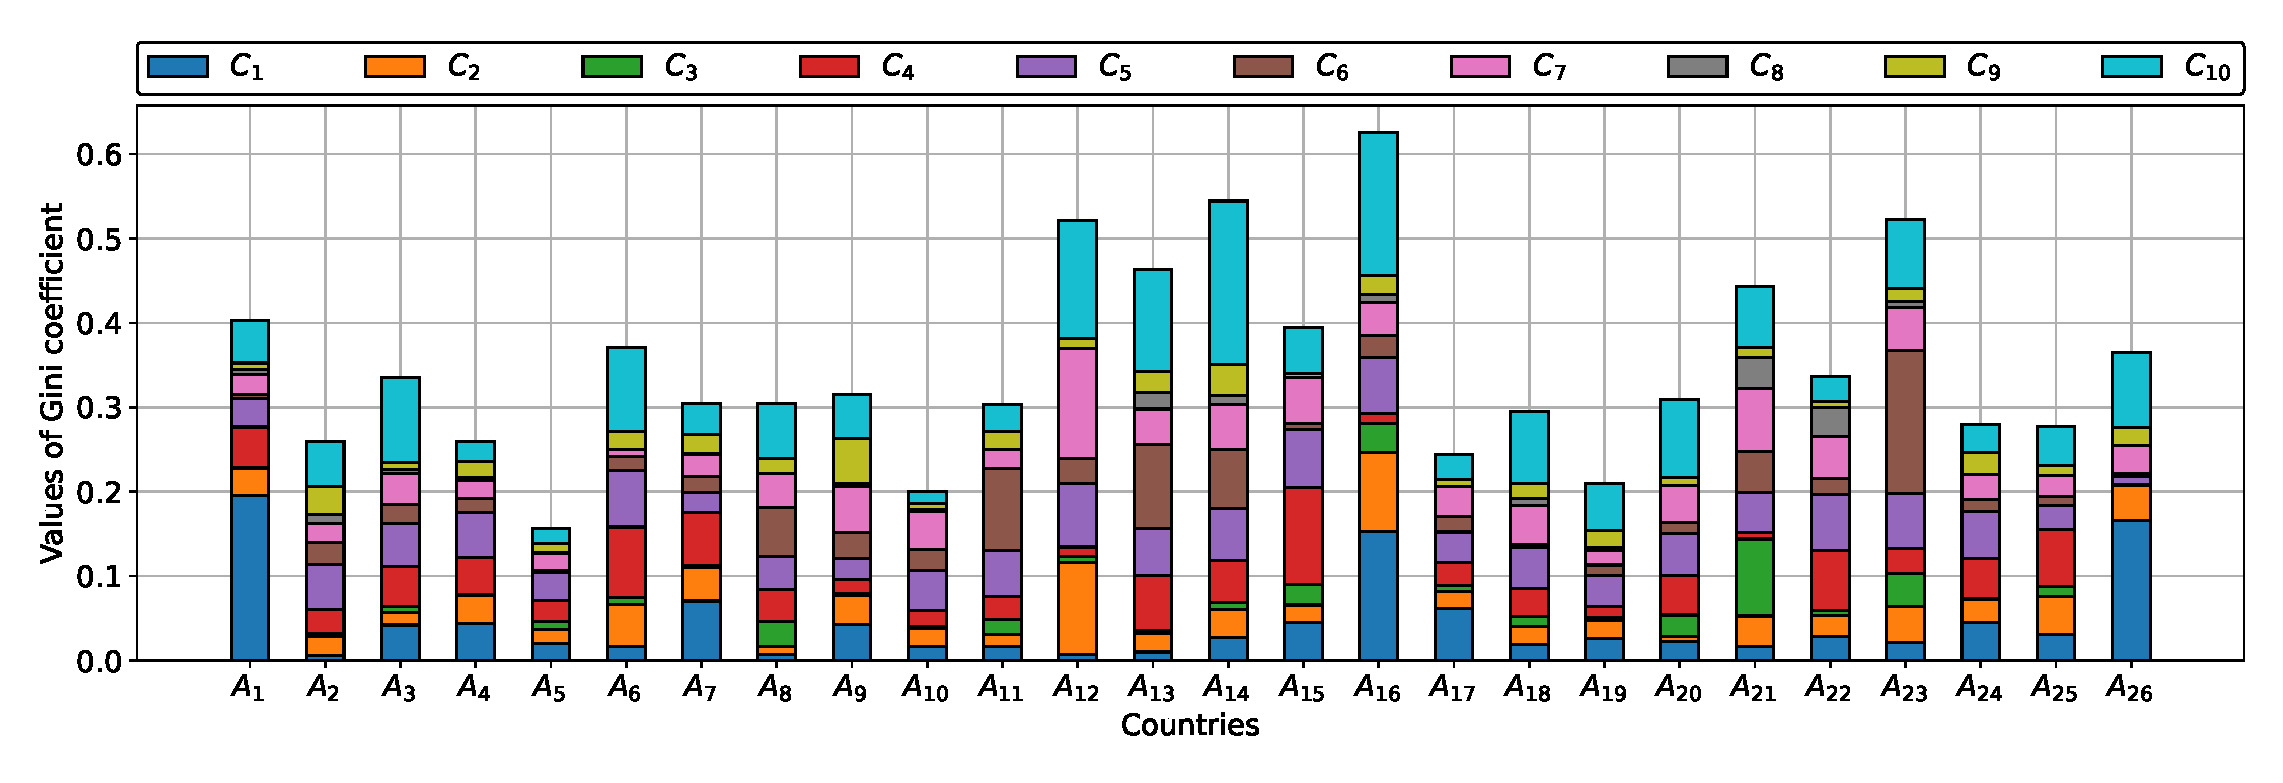
\includegraphics[width=0.8\linewidth]{dataset_Gini_coefficient.eps}
    \caption{Variability over the analyzed years 2015--2019 within the data values of particular criteria for evaluated countries measured by the Gini coefficient.}
    \label{fig:variabilityDataset}
\end{figure*}
%
The complementary analytical stage in this research was to determine the values and directions of variability among the criteria values for the countries analyzed over the five years surveyed. This procedure complements the approach involving countries' efficiencies with an analysis of the strength and direction of variability in the efficiency values provided by MCDAs as a final score over the years studied and enables simple identification of the most significant advances and decreases. Results, including the direction of variability and criteria sorted by descending order of its value, are displayed in Tables~\ref{tab:variabilityDatasetPart1} and~\ref{tab:variabilityDatasetPart2}. Direction $\uparrow$ indicates variability toward improvement for a criterion and represents an increase for the profit criterion and a decrease for cost. Conversely, direction $\downarrow$ denotes variability toward worsening and presents a decrease for the profit criterion and an increase for cost. The value variability in criteria for each country is also visualized in the cumulative column chart in Figure~\ref{fig:variabilityDataset}. Criterion variability results are not directly used to calculate efficiency variability and determine final rankings but provide additional information to identify upward or downward trends in evaluation criteria affecting individual country scores. For example, for Hungary ($A_{16}$), the highest variability in improving direction was observed for criteria $C_{10}$ (Population reporting occurrence of crime, violence, or vandalism in their area by poverty status) and $C_{1}$ (Overcrowding rate by poverty status). Moreover, the values of all criteria except $C_{9}$ (Share of buses and trains in total passenger transport) have improved over the five years analyzed. Therefore, the successive improvement in this country concerning the considered criteria is reflected in promotions in the received rankings. On the other hand, for the United Kingdom ($A_{26}$), there was a regression for as many as six assessment criteria, namely $C_{10}$ (Population reporting occurrence of crime, violence or vandalism in their area by poverty status), $C_{2}$ (Population living in households considering that they suffer from noise, by poverty status), $C_{7}$ (Population living in a dwelling with a leaking roof, damp walls, floors
or foundation or rot in window), $C_{9}$ (Share of buses and trains in total passenger transport), $C_{5}$ (Exposure to air pollution by
particulate matter) and $C_{3}$ (Settlement area per capita). Furthermore, for this country, improvement occurred for only two criteria, while the change direction for the other two criteria remained constant. Thus, the degradation observed for most of the criteria over the years evaluated contributed to the country's decrease in subsequent rankings.

\subsection{Effect of other variability measures on the final result of the DARIA-TOPSIS method}
\label{sec:ResultsBenchmarkVarMeasures}
%
\begin{figure*}[ht!]
    \centering
    \includegraphics[width=0.7\linewidth]{bar_chart_Variability_measures.eps}
    \caption{Comparison of rankings obtained using different variability measures in the DARIA-TOPSIS method.}
    \label{fig:compareVarMeasures}
\end{figure*}
%
The authors of this paper used the Gini coefficient to measure the variability in the performance of alternatives over given periods. However, other measures of variability also seem to be appropriate for application in the DARIA-TOPSIS method. Therefore, to validate and partially assess the results' robustness, the authors also explored other available variability measures. To confirm the stability of the solutions given by the Gini coefficient in the DARIA-TOPSIS method, a comparative analysis with four other measures of data variability was performed. The investigation included the following measures of variability: Standard deviation (Std), Statistical variance (Stat var), Entropy, and Coefficient of variation (Coeff var). Mentioned variability measures are described in detail in Supplementary Material in Appendix in sections A.5--A.8.
%
\begin{table}[H]
\centering
\caption{Comparison of rankings obtained with different variability measures.}
\label{tab:compareVarMeasures}
\resizebox{0.6\linewidth}{!}{
\begin{tabular}{lrrrrr} \toprule
$A_{i}$ & Gini & Std & Stat var & Entropy & Coeff var \\ \midrule
$A_{1}$ & 12 & 12 & 11 & 11 & 13 \\
$A_{2}$ & 26 & 25 & 25 & 25 & 25 \\
$A_{3}$ & 8 & 8 & 7 & 7 & 8 \\
$A_{4}$ & 7 & 7 & 5 & 5 & 12 \\
$A_{5}$ & 15 & 15 & 13 & 13 & 18 \\
$A_{6}$ & 3 & 2 & 3 & 3 & 2 \\
$A_{7}$ & 4 & 4 & 4 & 4 & 5 \\
$A_{8}$ & 24 & 24 & 24 & 24 & 26 \\
$A_{9}$ & 14 & 14 & 10 & 10 & 17 \\
$A_{10}$ & 11 & 11 & 9 & 9 & 14 \\
$A_{11}$ & 21 & 21 & 23 & 23 & 20 \\
$A_{12}$ & 17 & 17 & 20 & 20 & 9 \\
$A_{13}$ & 18 & 19 & 19 & 19 & 16 \\
$A_{14}$ & 13 & 13 & 16 & 16 & 11 \\
$A_{15}$ & 10 & 9 & 8 & 8 & 10 \\
$A_{16}$ & 6 & 6 & 12 & 12 & 4 \\
$A_{17}$ & 19 & 18 & 15 & 15 & 19 \\
$A_{18}$ & 5 & 5 & 6 & 6 & 6 \\
$A_{19}$ & 23 & 23 & 22 & 22 & 21 \\
$A_{20}$ & 22 & 22 & 21 & 21 & 23 \\
$A_{21}$ & 25 & 26 & 26 & 26 & 24 \\
$A_{22}$ & 16 & 16 & 18 & 18 & 15 \\
$A_{23}$ & 9 & 10 & 14 & 14 & 7 \\
$A_{24}$ & 1 & 1 & 1 & 1 & 1 \\
$A_{25}$ & 2 & 3 & 2 & 2 & 3 \\
$A_{26}$ & 20 & 20 & 17 & 17 & 22 \\ \bottomrule
\end{tabular}
}
\end{table}
%
The rankings of the assessed countries obtained using the DARIA-TOPSIS method with the Gini coefficient and the mentioned set of other variability measures are displayed on the bar chart in Figure~\ref{fig:compareVarMeasures} and provided in Table~\ref{tab:compareVarMeasures}. The obtained results confirm the high similarity of the rankings provided using the Gini coefficient with the reference rankings. Moreover, in the case of ranking obtained with application of the Gini coefficient, the highest similarity of compared rankings was found for comparison with Standard deviation. It is worth noting that all compared approaches consistently indicated alternative $A_{24}$, namely Finland, as the leader. It is significant because the leader is usually the most interesting alternative for decision-makers in multi-criteria decision analysis problems. To objectively confirm the reliability of the results, the authors determined Pearson correlation coefficient values between the compared rankings. The correlation results are displayed in Figure~\ref{fig:compareVarMeasuresCorrs}. 

%
\begin{figure}[H]
    \centering
    \includegraphics[width=0.7\linewidth]{pearson.eps}
    \caption{Pearson correlation between rankings obtained using different variability measures in the DARIA-TOPSIS method.}
    \label{fig:compareVarMeasuresCorrs}
\end{figure}
%

The results show the high convergence of the base ranking obtained with the DARIA-TOPSIS method using the Gini coefficient with rankings received using other variability measures. The highest correlation is observed for the comparison of the base ranking with the ranking obtained using Standard deviation as a measure of variance (0.9973). However, the comparison of the base ranking with the ranking received using Statistical variance and the Coefficient of variation also show high convergence confirmed by the Pearson correlation coefficient value (0.9480 for Statistical variance and Entropy and 0.9474 for Coefficient of variation). The conducted analysis comparing the authors' proposed approach with the application of the Gini coefficient as a measure of the variability of the results in the DARIA-TOPSIS method shows high convergence. It demonstrates the validity of the proposed approach and its potential usefulness in combination with different measures of variability. The observed differences between the results obtained using the compared measures of variability are negligible and show the potential of the proposed DARIA-TOPSIS method to be used with other measures of variability. However, full domain tests considering other decision problems in sustainability development are needed to fully validate the utility of explored measures of variability in the authors' proposed method. These investigations are planned as future works.


\subsection{Results of the DARIA-TOPSIS method performed for criteria groups representing dimensions perspective}
\label{sec:resultsDimensions}
As an example, one of the advantages of the DARIA-TOPSIS method is the ability to analyze alternatives against groups of criteria. In practice, it enables the definition and investigation of the implications for any semi-aggregated indicators.
%
%
\begin{figure*}[ht!]
    \centering
    \includegraphics[width=0.8\linewidth]{topsis_dims_Gini_coefficient.eps}
    \caption{Variability over the analyzed years 2015--2019 within the rankings of evaluated countries obtained by the DARIA-TOPSIS method for criteria dimensions.}
    \label{fig:RankingsVariabilityDimensionsTOPSIS}
\end{figure*}
%
%
\begin{table*}[ht!]
\centering
\caption{Variability over the analyzed years 2015--2019 within the rankings of evaluated countries obtained by TOPSIS measured by the Gini coefficient.}
\label{tab:variabilityRankingsDimensionsTOPSIS}
\resizebox{0.7\linewidth}{!}{
\begin{tabular}{lrclrclrc} \toprule
$A_{i}$ & Economic & Variability direction & $A_{i}$ & Environmental & Variability direction & $A_{i}$ & Social & Variability direction \\ \midrule
$A_{16}$ & 0.2386 & $\uparrow$ & $A_{12}$ & 0.0996 & $\uparrow$ & $A_{13}$ & 0.0855 & $\uparrow$ \\
$A_{12}$ & 0.0610 & $\uparrow$ & $A_{16}$ & 0.0622 & $\uparrow$ & $A_{26}$ & 0.0688 & $\downarrow$ \\
$A_{13}$ & 0.0493 & $\downarrow$ & $A_{23}$ & 0.0561 & $\uparrow$ & $A_{2}$ & 0.0666 & $\uparrow$ \\
$A_{21}$ & 0.0410 & $\uparrow$ & $A_{22}$ & 0.0555 & $\uparrow$ & $A_{15}$ & 0.0603 & $\uparrow$ \\
$A_{22}$ & 0.0285 & $\uparrow$ & $A_{21}$ & 0.0543 & $\downarrow$ & $A_{14}$ & 0.0529 & $\uparrow$ \\
$A_{23}$ & 0.0248 & $\uparrow$ & $A_{14}$ & 0.0424 & $\uparrow$ & $A_{21}$ & 0.0504 & $\uparrow$ \\
$A_{14}$ & 0.0222 & $\uparrow$ & $A_{15}$ & 0.0406 & $\downarrow$ & $A_{3}$ & 0.0479 & $\uparrow$ \\
$A_{11}$ & 0.0185 & $\downarrow$ & $A_{11}$ & 0.0398 & $\uparrow$ & $A_{1}$ & 0.0477 & $\uparrow$ \\
$A_{2}$ & 0.0183 & $\downarrow$ & $A_{2}$ & 0.0397 & $\uparrow$ & $A_{12}$ & 0.0475 & $\uparrow$ \\
$A_{19}$ & 0.0182 & $\uparrow$ & $A_{8}$ & 0.0362 & $\downarrow$ & $A_{18}$ & 0.0446 & $\uparrow$ \\
$A_{18}$ & 0.0182 & $\uparrow$ & $A_{13}$ & 0.0330 & $\uparrow$ & $A_{11}$ & 0.0400 & $\uparrow$ \\
$A_{3}$ & 0.0166 & $\uparrow$ & $A_{3}$ & 0.0261 & $\uparrow$ & $A_{22}$ & 0.0383 & $\uparrow$ \\
$A_{6}$ & 0.0158 & $\downarrow$ & $A_{26}$ & 0.0239 & $\downarrow$ & $A_{23}$ & 0.0373 & $\uparrow$ \\
$A_{8}$ & 0.0143 & $\uparrow$ & $A_{20}$ & 0.0209 & $\downarrow$ & $A_{6}$ & 0.0355 & $\uparrow$ \\
$A_{15}$ & 0.0130 & $\uparrow$ & $A_{19}$ & 0.0190 & $\uparrow$ & $A_{19}$ & 0.0296 & $\uparrow$ \\
$A_{9}$ & 0.0127 & $\uparrow$ & $A_{10}$ & 0.0187 & $\uparrow$ & $A_{9}$ & 0.0296 & $\downarrow$ \\
$A_{20}$ & 0.0123 & $\uparrow$ & $A_{4}$ & 0.0167 & $\downarrow$ & $A_{8}$ & 0.0276 & $\downarrow$ \\
$A_{25}$ & 0.0119 & $\downarrow$ & $A_{9}$ & 0.0167 & $\downarrow$ & $A_{16}$ & 0.0234 & $\uparrow$ \\
$A_{7}$ & 0.0119 & $\uparrow$ & $A_{25}$ & 0.0158 & $\downarrow$ & $A_{17}$ & 0.0232 & $\downarrow$ \\
$A_{4}$ & 0.0116 & $\downarrow$ & $A_{1}$ & 0.0127 & $\uparrow$ & $A_{25}$ & 0.0229 & $\downarrow$ \\
$A_{1}$ & 0.0105 & $\downarrow$ & $A_{18}$ & 0.0119 & $\downarrow$ & $A_{7}$ & 0.0213 & $\uparrow$ \\
$A_{17}$ & 0.0083 & $\uparrow$ & $A_{7}$ & 0.0112 & $\downarrow$ & $A_{24}$ & 0.0212 & $\uparrow$ \\
$A_{5}$ & 0.0075 & $\uparrow$ & $A_{17}$ & 0.0108 & $\downarrow$ & $A_{20}$ & 0.0160 & $\uparrow$ \\
$A_{26}$ & 0.0069 & $\downarrow$ & $A_{6}$ & 0.0077 & $\uparrow$ & $A_{4}$ & 0.0104 & $\downarrow$ \\
$A_{24}$ & 0.0053 & $\downarrow$ & $A_{5}$ & 0.0072 & $\downarrow$ & $A_{10}$ & 0.0082 & $\downarrow$ \\
$A_{10}$ & 0.0048 & $\uparrow$ & $A_{24}$ & 0.0024 & $\uparrow$ & $A_{5}$ & 0.0063 & $\uparrow$ \\ \bottomrule
\end{tabular}
}
\end{table*}
%

%
\begin{table*}[ht!]
\centering
\caption{Aggregated efficiency of performance values and rankings covering 2015--2019 calculated applying the DARIA-TOPSIS method for criteria dimensions.}
\label{tab:FinalResultsIndexTOPSIS}
\resizebox{0.6\linewidth}{!}{
\begin{tabular}{lrrrrrr} \toprule
 & \multicolumn{3}{c}{Efficiency} & \multicolumn{3}{c}{Rankings} \\
$A_{i}$ & Economic & Environmental & Social & Economic & Environmental & Social \\ \midrule
$A_{1}$ & 0.5089 & 0.6440 & 0.5609 & 14 & 6 & 17 \\
$A_{2}$ & 0.2943 & 0.4210 & 0.2675 & 25 & 23 & 26 \\
$A_{3}$ & 0.5732 & 0.5192 & 0.7414 & 7 & 21 & 3 \\
$A_{4}$ & 0.5541 & 0.6183 & 0.6625 & 10 & 9 & 9 \\
$A_{5}$ & 0.5610 & 0.5702 & 0.5505 & 9 & 15 & 18 \\
$A_{6}$ & 0.5962 & 0.7822 & 0.7403 & 6 & 2 & 4 \\
$A_{7}$ & 0.6331 & 0.6352 & 0.7072 & 3 & 7 & 6 \\
$A_{8}$ & 0.4089 & 0.4202 & 0.3600 & 21 & 24 & 24 \\
$A_{9}$ & 0.5497 & 0.5694 & 0.5416 & 11 & 16 & 19 \\
$A_{10}$ & 0.5966 & 0.6285 & 0.4876 & 5 & 8 & 22 \\
$A_{11}$ & 0.3397 & 0.4370 & 0.6025 & 24 & 22 & 12 \\
$A_{12}$ & 0.4174 & 0.5720 & 0.6310 & 20 & 14 & 11 \\
$A_{13}$ & 0.2056 & 0.6603 & 0.6405 & 26 & 5 & 10 \\
$A_{14}$ & 0.4938 & 0.6677 & 0.5623 & 16 & 4 & 16 \\
$A_{15}$ & 0.5348 & 0.5899 & 0.6748 & 13 & 13 & 8 \\
$A_{16}$ & 0.6050 & 0.5927 & 0.7397 & 4 & 12 & 5 \\
$A_{17}$ & 0.5392 & 0.5646 & 0.4718 & 12 & 17 & 23 \\
$A_{18}$ & 0.5695 & 0.5975 & 0.7493 & 8 & 11 & 2 \\
$A_{19}$ & 0.3650 & 0.3958 & 0.5988 & 23 & 25 & 14 \\
$A_{20}$ & 0.4483 & 0.5369 & 0.5042 & 19 & 20 & 21 \\
$A_{21}$ & 0.3660 & 0.1928 & 0.5056 & 22 & 26 & 20 \\
$A_{22}$ & 0.4734 & 0.5420 & 0.5925 & 17 & 19 & 15 \\
$A_{23}$ & 0.4672 & 0.5637 & 0.8056 & 18 & 18 & 1 \\
$A_{24}$ & 0.9279 & 0.7966 & 0.6750 & 1 & 1 & 7 \\
$A_{25}$ & 0.7798 & 0.7489 & 0.6009 & 2 & 3 & 13 \\
$A_{26}$ & 0.4953 & 0.6053 & 0.3421 & 15 & 10 & 25 \\ \bottomrule
\end{tabular}
}
\end{table*}
%

For this purpose, three additional models were developed. A model containing criteria $C_{1}$, $C_{3}$, and $C_{7}$ was created to assess sustainability for the economic dimension, a model including criteria $C_{2}$, $C_{5}$, $C_{6}$, and $C_{8}$ was constructed for the environmental dimension, and a model for the social dimension incorporated criteria $C_{4}$, $C_{9}$, and $C_{10}$.

In this study, according to Table~\ref{tab:criteria} containing problem structuring, the following analysis was realized for criteria grouped into three distinct dimensions. The evaluation procedure performed for the complete data was repeated for individual models containing criteria belonging to three main dimensions: economic, environmental, and social. The variability of the analyzed countries' rankings concerning particular criteria dimensions is visualized in Figure~\ref{fig:RankingsVariabilityDimensionsTOPSIS}. In addition, the values and directions of variability are included in Table~\ref{tab:variabilityRankingsDimensionsTOPSIS}. By far, the most extensive range of variability is observed in $A_{16}$ (Hungary) for the economic dimension, which causes advancement over the years analyzed. 

Final results, including efficiency and ranks values calculated applying the DARIA-TOPSIS method for particular criteria dimensions, are contained in Table~\ref{tab:FinalResultsIndexTOPSIS}. In the model with economic criteria, Finland ($A_{24}$) was indicated as the leader, followed by Sweden ($A_{25}$). The worst scored alternatives in the economic dimension are $A_{13}$ (Latvia) and $A_{2}$ (Bulgaria). The highest-ranked countries in terms of environmental dimension were $A_{24}$ (Finland) and $A_{6}$ (Estonia) and in last place was $A_{21}$ (Romania). Concerning social criteria
$A_{23}$ (Slovakia) and $A_{3}$ (Czechia) demonstrated the highest scores, while $A_{26}$ (United Kingdom) took second-to-last place and a large variability towards degradation in rankings, besides $A_{2}$ Bulgaria showed the worst score. The evaluation of the dynamics in efficiencies' variability showed that in the case of the economic dimension, the most significant progress was demonstrated by $A_{16}$ (Hungary), $A_{12}$ (Italy), and $A_{21}$ (Romania), for the environmental dimension $A_{12}$ (Italy), $A_{16}$ (Hungary), $A_{23}$ (Slovenia) and $A_{22}$ (Slovakia), however, for social dimension $A_{13}$ (Latvia) and $A_{2}$ (Bulgaria) showed the most remarkable advancement.

\subsection{The DARIA-TOPSIS method based detailed alternatives analysis}
\label{sec:resultsDiscussion}
As proved in the above theoretical and practical considerations, the DARIA-TOPSIS method represents a successful attempt considering data variability in multi-criteria assessment, and practical research demonstrates its usefulness in the sustainable cities and society domain. The main advantage of the proposed approach is taking into account the dynamics of the variability of alternatives' efficiency values over investigated time.

The DARIA-TOPSIS method, designed for calculating the value and direction of efficiency variability, may be applied to determine the dynamics of results variability in particular years. In contrast to classical methods, it allows accounting for variability in alternatives' performance over time analyzed on the final overall evaluation ranking. The calculation of final rankings is based on more information, which includes the TOPSIS efficiency's values of alternatives for particular years and their variability reflecting progress or regression. Thus, this strategy results in rankings different from classical methods.
A country getting the same place in both the classical TOPSIS method and the DARIA-TOPSIS method indicates a stable situation for a given alternative. Obtaining a worse score for DARIA adapted for TOPSIS than the results provided by classical TOPSIS for individual years signals a tendency for the country's situation to worsen, which is inconsistent with the sustainability paradigm. On the other hand, a better score of the DARIA-TOPSIS method than the classical approach result expresses that the country shows improvements indicative of expected development.

The proposed methodology makes it possible to incorporate even slight differences in efficiency values for the years examined. An alternative may rank the same for all years, and after taking into account the variability in subsequent efficiencies for following years by the DARIA-TOPSIS method, it finally ranks higher. Such a situation is demonstrated for $A_{18}$ (Austria) by the DARIA-TOPSIS method. It is caused by improvement of efficiency in subsequent years. On the other hand, successive improvement in efficiency does not always guarantee promotion in the final ranking. For example, it is the case of $A_{2}$ (Bulgaria), which, despite the improvement in efficiency in the DARIA-TOPSIS method, was finally ranked 26th, although it was 25th in all years. This situation is caused by the fact that other alternatives from the evaluated set obtained higher values of aggregated efficiency and overtook this alternative. Thus, the final score also depends on the scores of the other alternatives.

Table~\ref{tab:FinlandTrends} displays trends in sustainability indicators published by Eurostat for Finland~\cite{eurostat2021, brochureEurostat2021, SDGandME2021} beginning from most significant criterion. It is clear that during the examined period in Finland, there was an improvement in the form of reduction of air pollution $C_{5}$ (environmental dimension), decrease in the rate of deaths due to road traffic $C_{4}$, improvement of safety $C_{10}$ (social dimension), housing standards $C_{7}$ (economic dimension), increase in the public transport fleet $C_{9}$ (social dimension), increase in the share of recycling of municipal waste $C_{6}$ (environmental dimension). On the other hand, deterioration was observed only in three social indicators, namely an increase in overcrowding rate $C_{1}$, disturbance by noise $C_{2}$, and decrease in settlement area per capita $C_{3}$. Second, in the TOPSIS ranking is Sweden ($A_{25}$), for which trends in changes in criteria values are shown in Table~\ref{tab:SwedenTrends}. In the case of Sweden, there has been a reduction in road accident deaths, with the $C_{4}$ indicator in 2019 taking the lowest value over the five years studied, reaching the lowest value of all countries assessed. In addition, there has been a reduction in air pollution $C_{5}$, an improvement in housing $C_{7}$, and an increase in public transport $C_{9}$. Unfortunately, the resident safety index $C_{10}$ worsens as more crimes are reported, noise pollution $C_{2}$, and overcrowding rate $C_{1}$ also increases. However, the settlement area index $C_{3}$ decreased, and the recycling rate of municipal waste in 2018-2019 was lower than in 2015-2017. The described deterioration contributed to Sweden's decline from the leading position in 2015 to the second position in the remaining years.
Third place in ranking provided by the DARIA-TOPSIS method took Estonia ($A_{6}$), Ireland ($A_{7}$) ranked fourth, and Austria ($A_{18}$) was ranked fifth. 

In the United Kingdom, with criteria performance values displayed in Table~\ref{tab:UKTrends}, the crime rate $C_{10}$ has steadily increased for five consecutive years since 2015, contributing to a significant decline in population safety (social). The number of people living in noise pollution $C_{2}$ (environmental) and the number of people with poor housing $C_{7}$ (economic) are increasing, and the number of accessible public transport vehicles $C_{9}$ (social) is decreasing. There is no decrease in air pollution $C_{5}$, and settlement per capita decreases $C_{3}$ (economic). The number of traffic fatalities is stable and is one of the lowest compared to other countries. Reductions in overcrowding (economic) and an increase in the recycling rate of municipal (environmental) waste are not enough to prevent the United Kingdom from falling in rankings. Deterioration for social criteria $C_{9}$ and $C_{10}$ contributed to the fact that the United Kingdom's overall evaluation using the DARIA-TOPSIS method in the social dimension was in the penultimate place. However, in the economic dimension, it is fifteenth, and in the environmental dimension tenth.
%
% Finland
\begin{table}[H]
\centering
\caption{Trends in sustainability indicators published by Eurostat for Finland.}
\label{tab:FinlandTrends}
\resizebox{\linewidth}{!}{
\begin{tabular}{lrrrrr
>{\centering\arraybackslash}p{3cm}
} \toprule
Finland & 2015 & 2016 & 2017 & 2018 & 2019 & Trend (Improvement $\uparrow$, Worsening  $\downarrow$, Stability $=$) \\ \midrule
$C_{5}$ & 6 & 5.7 & 4.9 & 6.4 & 5.1 & $\uparrow$ \\
$C_{4}$ & 4.9 & 4.7 & 4.3 & 4.3 & 3.8 & $\uparrow$ \\
$C_{10}$ & 7.3 & 6.5 & 6.2 & 7 & 6.4 & $\uparrow$ \\
$C_{7}$ & 4.4 & 4.7 & 4.2 & 4.6 & 4.1 & $\uparrow$ \\
$C_{9}$ & 15 & 17.5 & 15.8 & 15.8 & 16.1 & $\uparrow$ \\
$C_{6}$ & 40.6 & 42 & 40.5 & 42.3 & 43.5 & $\uparrow$ \\
$C_{8}$ & 85 & 85 & 85 & 85 & 85 & $=$ \\
$C_{1}$ & 6.7 & 6.6 & 6.1 & 7.3 & 7.7 & $\downarrow$ \\
$C_{2}$ & 11.7 & 12 & 12.5 & 13.4 & 12.8 & $\downarrow$ \\
$C_{3}$ & 2458.7 & 2458.7 & 2458.7 & 2447.6 & 2447.6 & $\downarrow$ \\ \bottomrule
\end{tabular}
}
\end{table}
%
% Sweden
\begin{table}[H]
\centering
\caption{Trends in sustainability indicators published by Eurostat for Sweden.}
\label{tab:SwedenTrends}
\resizebox{\linewidth}{!}{
\begin{tabular}{lrrrrr
>{\centering\arraybackslash}p{3cm}
} \toprule
Sweden & 2015 & 2016 & 2017 & 2018 & 2019 & Trend (Improvement $\uparrow$, Worsening  $\downarrow$, Stability $=$ \\ \midrule
$C_{4}$ & 2.6 & 2.7 & 2.5 & 3.2 & 2.2 & $\uparrow$ \\
$C_{5}$ & 6.1 & 5.6 & 5.4 & 6.2 & 5.8 & $\uparrow$ \\
$C_{7}$ & 7.7 & 7.4 & 7 & 7.8 & 7 & $\uparrow$ \\
$C_{9}$ & 16.8 & 16.5 & 16.7 & 16.9 & 17.7 & $\uparrow$ \\
$C_{8}$ & 95 & 95 & 95 & 95 & 95 & $=$ \\
$C_{10}$ & 10.9 & 12.7 & 13 & 14.4 & 13 & $\downarrow$ \\
$C_{2}$ & 12.6 & 17.1 & 16.9 & 17 & 17 & $\downarrow$ \\
$C_{1}$ & 13.9 & 14.4 & 13.5 & 15.2 & 15.6 & $\downarrow$ \\
$C_{3}$ & 2343.8 & 2343.8 & 2343.8 & 2223 & 2223 & $\downarrow$ \\
$C_{6}$ & 47.5 & 48.4 & 46.8 & 45.8 & 46.6 & $\downarrow$ \\ \bottomrule
\end{tabular}
}
\end{table}
%
% United Kingdom
\begin{table}[H]
\centering
\caption{Trends in sustainability indicators published by Eurostat for United Kingdom.}
\label{tab:UKTrends}
\resizebox{\linewidth}{!}{
\begin{tabular}{lrrrrr
>{\centering\arraybackslash}p{3cm}
} \toprule
United Kingdom & 2015 & 2016 & 2017 & 2018 & 2019 & Trend (Improvement $\uparrow$, Worsening  $\downarrow$, Stability $=$ \\ \midrule
$C_{10}$ & 16.6 & 16.8 & 20.3 & 24.2 & 24.2 & $\downarrow$ \\
$C_{2}$ & 16.5 & 17 & 17.3 & 19.8 & 19.8 & $\downarrow$ \\
$C_{7}$ & 14.8 & 16.4 & 17 & 17.6 & 17.6 & $\downarrow$ \\
$C_{9}$ & 14.1 & 13.5 & 13.3 & 12.9 & 12.6 & $\downarrow$ \\
$C_{5}$ & 10 & 10.4 & 9.9 & 10.1 & 10.2 & $\downarrow$ \\
$C_{3}$ & 430.5 & 430.5 & 430.5 & 426.9 & 426.9 & $\downarrow$ \\
$C_{4}$ & 2.8 & 2.8 & 2.8 & 2.8 & 2.8 & $=$ \\
$C_{8}$ & 100 & 100 & 100 & 100 & 100 & $=$ \\
$C_{1}$ & 7.3 & 8 & 3.4 & 4.8 & 4.8 & $\uparrow$ \\
$C_{6}$ & 43.3 & 44 & 43.8 & 44.1 & 44.1 & $\uparrow$ \\ \bottomrule
\end{tabular}
}
\end{table}
%

The research results demonstrate high correlations between the different MCDA methods applied for sustainable cities and society assessment. This fact proves the high robustness of the TOPSIS approach adapted for the DARIA-TOPSIS method proposed in this research. The proposed approach may find application primarily in problems where the analysis based on single results is insufficient, and it is essential to take into account the dynamics of change over the years, i.e., in the areas of assessing the sustainable development of, among others, countries, cities, and regions and beyond.

\section{Conclusions}
\label{sec:concl}

This paper presents a new MCDA method named the DARIA-TOPSIS. From a methodical point of view, the proposed approach extends the classical MCDA paradigm of evaluating the current set of alternatives to the dynamic approach. The DARIA-TOPSIS method enables evaluating alternatives, taking into account a set of efficiencies of options from any number of periods of analyzed time. As demonstrated in the paper, this method has many advantages. The DARIA-TOPSIS method, besides the time-based overall evaluation of alternatives, also provides detailed efficiencies and rankings of alternatives for all investigated periods, which gives the user additional analytical capabilities. Furthermore, the DARIA-TOPSIS method enables temporal assessment of both the model containing the full criteria tree and criteria groups. Besides, in addition to determining the dynamics and direction of variation of efficiencies, the proposed method provides the possibility of analogous evaluation of the variability of criteria for alternatives in particular periods. Meanwhile, the advantage of the proposed DARIA-TOPSIS method is the clarity and simplicity of the algorithm. It also does not require additional data compared to the classical TOPSIS method (as it occurs in other approaches). Furthermore, the algorithm of the proposed method is fully automated, having low computational complexity even for a large number of alternatives and criteria. An additional advantage of the proposed method is that it is easily adaptable to other MCDA methods. It is also worth emphasizing that the provided DARIA TOPSIS algorithm retains the complete analytical properties of both the underlying TOPSIS method and the original data set.

Practical contribution is provided in the form of DARIA-TOPSIS method-based structured framework supporting sustainable cities and communities assessment in the EU countries. The research and analysis performed allow to conclude that the proposed framework has clearly demonstrated its usefulness and added value in providing a holistic view of the overall and multistage sustainability assessment process. The conducted research demonstrated that in the case of multi-dimensional sustainability assessment, the final results are influenced by many factors. Among them are factors such as the current evaluation of the alternatives for the most recent period, the dynamics of the variability of the results during the investigated past years, and the direction of this variability. Furthermore, due to the fact that the framework is based on MCDA assumptions, it inherits all the analytical potential of this group of methods. The research carried out in this paper for groups of criteria, and the analysis of selected alternatives shows this clearly. The authors also provided a technical contribution - complete pseudo-code and Python code of the newly developed DARIA-TOPSIS method. As a result, the full implementation that allows a broad audience, including other scientists, to use it for their research is publicly available~\cite{dariagithub2022}. Provided implementation includes the DARIA TOPSIS method code with variability measures applied in this paper. Besides, it includes the TOPSIS method and other supporting methods such as objective weighting methods, normalization techniques, and correlation coefficients necessary to perform a complete multi-criteria temporal assessment procedure.    

When summarizing the present research, the methodological and practical contributions of the paper are: 

\begin{itemize}
    \item {Development of a new MCDA method called Data vARIability Assessment Technique for Order of Preference by Similarity to Ideal Solution (the DARIA-TOPSIS method), taking into account multiple periods with data, its variability, and aggregation to a single final ranking.}
    \item {Complete DARIA-TOPSIS method-based framework supporting multi-period evaluation of sustainable cities and societies in EU countries, and multi-perspective analysis of the modeling results of the sustainability assessment in terms of both overall and criteria groups (economic, environmental and social) perspectives evaluation, and detailed alternatives analysis as well.}
    \item {Complete algorithms, and pseudo-codes for the DARIA-TOPSIS method fully available to a wide audience.}
\end{itemize}

The presented research initiated several directions for further work and exposed the arising research questions. Future research could include using other measures of variability and its comparison with the Gini coefficient and exploring other MCDA methods in the time-based aggregation domain. An interesting direction for further work seems to be the construction of a framework for the selected methods of the European school, taking into account both methods giving quantitative results, such as PROMETHEE II, and qualitative results, such as the ELECTRE family-based methods. Besides, following recent developments of MCDA methods, adapting fuzzy extensions of classical methods to a dynamic approach taking into account data variability seems to be a promising research field. 

\appendix
\label{sec:app}
\section{The PRISMA Methodology}
\label{sec:appPRISMA}
This section presents the PRISMA bibliographic literature review method. It is one of the recognized methodologies to perform a literature review that the authors of this article adapted to obtain relevant literature examples in the Literature review section. The following stages of the PRISMA methodology are presented below.

\begin{itemize}
    \item {Step 1. Identify the aim of the research.}
    \item {Step 2. Define the database for the selection of papers.}
    \item {Step 3. Define conditions of papers selection.}
    \item {Step 4. Introduce the categorization for papers' analysis in the domain of the research.}
\end{itemize}

The first stage is discussed in the Introduction section, which highlights the relationship of the authors' research to the assessment of sustainable cities and society. In the second stage, the authors selected the Scopus database as a source of relevant articles due to a large number of publishers, a variety of collections of papers, and a large number of journals with high citation indexes. In the next step, the authors defined keywords in the scope of the article topic to adequately select sample papers. The following are the keywords divided into different groups that the authors used to search for articles necessary for the literature review. The combinations of keywords used in the paper searching procedure are additionally displayed in Table~\ref{tab:prismakeywords}.

\begin{itemize}
    \item {Group 1: MCDA, multi-criteria decision analysis, multi-criteria decision aid, multi-criteria assessment/evaluation to limit the search to papers with any MCDA method;}
    \item {Group 2: Sustainable development, sustainability to gather papers focused on smart, sustainable development;}
    \item {Group 3: Society, smart city, cities to collect papers focused on development of urban areas and cities.}
\end{itemize}

\begin{table}[H]
\centering
\caption{Keywords used in the paper searching procedure.}
\label{tab:prismakeywords}
\begin{tabular}{lp{5cm}} \toprule
Group & Keywords \\ \midrule
Group 1 & MCDA \textbf{OR} multi-criteria decision analysis \textbf{OR} multi-criteria decision aid \textbf{OR} multi-criteria assessment \textbf{OR} multi-criteria evaluation \\
\textbf{AND} &  \\
Group 2 & sustainable \textbf{OR} sustainability \textbf{OR} sustainable development \textbf{OR} smart \\
\textbf{AND} &  \\
Group 3 & society \textbf{OR} smart cities \textbf{OR} cities \textbf{OR} urban \textbf{OR} urban areas \textbf{OR} regions \textbf{OR} management \\ \bottomrule
\end{tabular}
\end{table}

%
\begin{figure}[H]
    \centering
    \includegraphics[width=0.7\linewidth]{PRISMA_v102.png}
    \caption{The stages of the PRISMA methodology.}
    \label{fig:PRISMA}
\end{figure}
%
Figure~\ref{fig:PRISMA} displays a framework containing the various steps included in the PRISMA procedure with the effect of searching in the form of a number of papers collected and excluded in each stage.

\section{Benchmarking the TOPSIS method results for investigated periods with other selected MCDA methods}
\label{sec:app1}

Since many authors indicate the necessity of benchmarking results from different approaches~\cite{cinelli2020support, cinelli2022recommending}, the authors decided to benchmark the results of the TOPSIS method received for each investigated period with two other MCDA methods. Rankings given by the TOPSIS method were compared with reference MCDA methods, namely VIKOR and COMET. The outcomes are displayed on radar charts separately for the MCDA methods used in Figure~\ref{fig:radars}.

%
\begin{figure}[H]
\centering
\quad
\subfloat[][VIKOR]{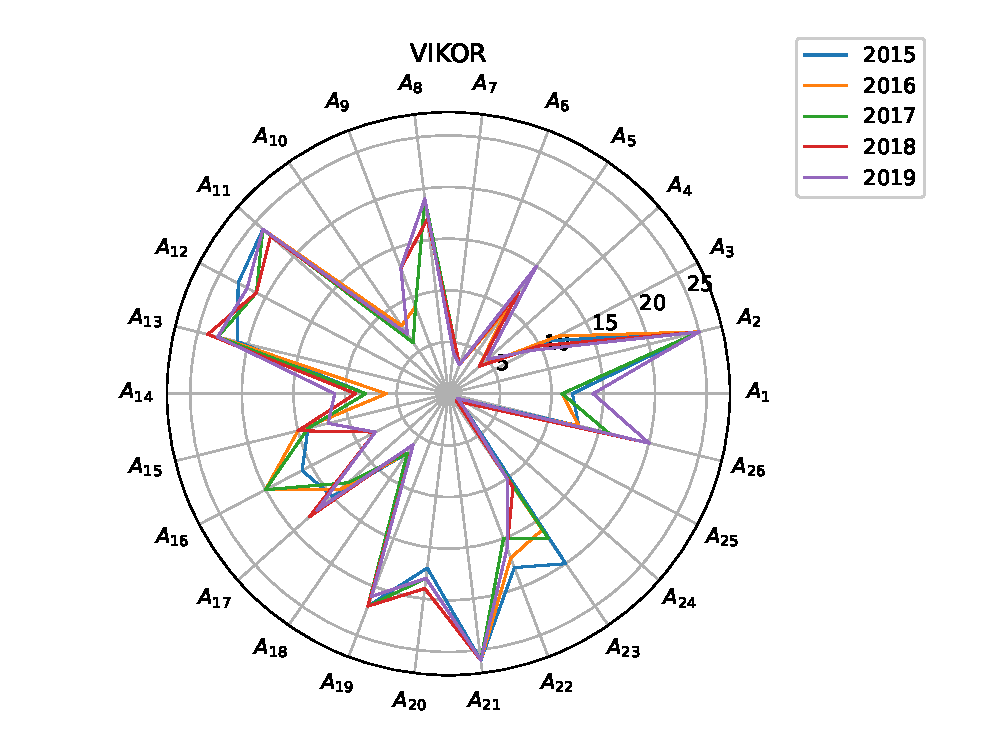
\includegraphics[width=\linewidth]{radar_vikor.eps}}
\quad
\subfloat[][COMET]{\includegraphics[width=\linewidth]{radar_comet.eps}}
\caption{Comparison of rankings of evaluated countries obtained by benchmarking MCDA methods for 2015-2019.}
\label{fig:radars}
\end{figure}
%
%
\begin{figure*}[ht!]
\centering
\quad
\subfloat[][2015]{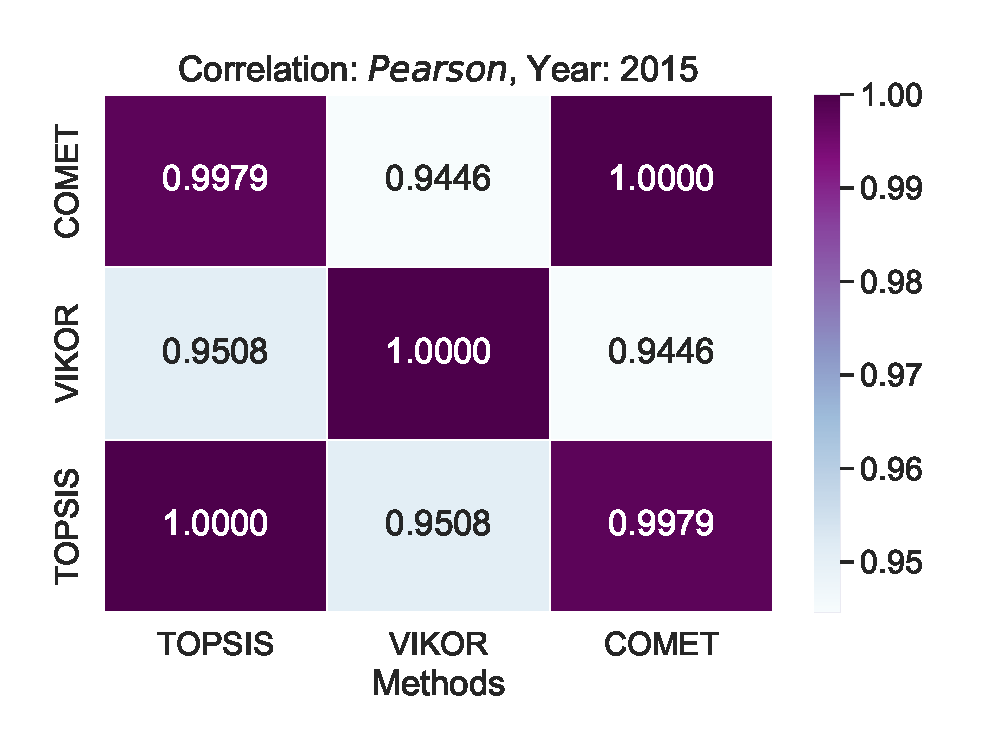
\includegraphics[width=0.25\linewidth]{pearson_2015.eps}}
\subfloat[][2016]{\includegraphics[width=0.25\linewidth]{pearson_2016.eps}}
\subfloat[][2017]{\includegraphics[width=0.25\linewidth]{pearson_2017.eps}}
\quad
\subfloat[][2018]{\includegraphics[width=0.25\linewidth]{pearson_2018.eps}}
\subfloat[][2019]{\includegraphics[width=0.25\linewidth]{pearson_2019.eps}}
\caption{Pearson's correlation coefficient values between rankings for considered years 2015--2019.}
\label{fig:correlations}
\end{figure*}
%
Rankings obtained for each investigated year were compared using Pearson's correlation coefficient. The results of the rankings similarity study are visualized in Figure~\ref{fig:correlations}. The highest convergence for the five years analyzed was noticed between the rankings provided by TOPSIS and COMET. Rankings obtained by the VIKOR method showed a higher correlation with TOPSIS than with COMET. The results obtained show a high degree of rankings' convergence, proving that the TOPSIS method produces reliable results and constitutes an appropriate method for performing analysis based on the DARIA-TOPSIS method. High correlation confirms the reliability of TOPSIS results.

\section*{Acknowledgments}
The work was supported by the project financed within the framework of the program of the Minister of Science and Higher Education under the name “Regional Excellence Initiative” in the years 2019-2022, Project Number 001/RID/2018/19; the amount of financing: PLN 10.684.000,00 (J.W. and A.B.) and by the National Science Centre, Decision No. 2018/29/B/HS4/02725 (W.S.).

\bibliography{mybibfile}

\end{document}